%% (Master) Thesis template
% Template version used: v1.4
%
% Largely adapted from Adrian Nievergelt's template for the ADPS
% (lecture notes) project.

\PassOptionsToPackage{dvipsnames}{xcolor}

%% We use the memoir class because it offers a many easy to use features.
\documentclass[11pt,a4paper,titlepage]{memoir}

%% Packages
%% ========

%% LaTeX Font encoding -- DO NOT CHANGE
\usepackage[OT1]{fontenc}

%% Babel provides support for languages.  'english' uses British
%% English hyphenation and text snippets like "Figure" and
%% "Theorem". Use the option 'ngerman' if your document is in German.
%% Use 'american' for American English.  Note that if you change this,
%% the next LaTeX run may show spurious errors.  Simply run it again.
%% If they persist, remove the .aux file and try again.
\usepackage[english]{babel}

%% Input encoding 'utf8'. In some cases you might need 'utf8x' for
%% extra symbols. Not all editors, especially on Windows, are UTF-8
%% capable, so you may want to use 'latin1' instead.
\usepackage[utf8]{inputenc}

%% This changes default fonts for both text and math mode to use Herman Zapfs
%% excellent Palatino font.  Do not change this.
\usepackage[sc]{mathpazo}

%% The AMS-LaTeX extensions for mathematical typesetting.  Do not
%% remove.
\usepackage{amsmath,amssymb,amsfonts,mathrsfs}

%% NTheorem is a reimplementation of the AMS Theorem package. This
%% will allow us to typeset theorems like examples, proofs and
%% similar.  Do not remove.
%% NOTE: Must be loaded AFTER amsmath, or the \qed placement will
%% break
\usepackage[amsmath,thmmarks]{ntheorem}

%% LaTeX' own graphics handling
\usepackage{graphicx}
\graphicspath{ {Graphics/} } %tell package where to find graphics


%% We unfortunately need this for the Rules chapter.  Remove it
%% afterwards; or at least NEVER use its underlining features.
\usepackage{soul}

%% This allows you to add .pdf files. It is used to add the
%% declaration of originality.
\usepackage{pdfpages}

\usepackage{xspace}

\usepackage{capt-of}

\usepackage{float}

\usepackage[section]{placeins}

\usepackage{subfig}

\usepackage[square, comma, sort&compress, numbers]{natbib}
%% Some more packages that you may want to use.  Have a look at the
%% file, and consult the package docs for each.
%% See the TeXed file for more explanations

%% [OPT] Multi-rowed cells in tabulars
%\usepackage{multirow}

%% [REC] Intelligent cross reference package. This allows for nice
%% combined references that include the reference and a hint to where
%% to look for it.
\usepackage{varioref}

%% [OPT] Easily changeable quotes with \enquote{Text}
%\usepackage[german=swiss]{csquotes}

%% [REC] Format dates and time depending on locale
\usepackage{datetime}

%% [OPT] Provides a \cancel{} command to stroke through mathematics.
%\usepackage{cancel}

%% [NEED] This allows for additional typesetting tools in mathmode.
%% See its excellent documentation.
\usepackage{mathtools}

%% [ADV] Conditional commands
%\usepackage{ifthen}

%% [OPT] Manual large braces or other delimiters.
%\usepackage{bigdelim, bigstrut}

%% [REC] Alternate vector arrows. Use the command \vv{} to get scaled
%% vector arrows.
\usepackage[h]{esvect}

%% [NEED] Some extensions to tabulars and array environments.
\usepackage{array}

%% [OPT] Postscript support via pstricks graphics package. Very
%% diverse applications.
%\usepackage{pstricks,pst-all}

%% [?] This seems to allow us to define some additional counters.
%\usepackage{etex}

%% [ADV] XY-Pic to typeset some matrix-style graphics
%\usepackage[all]{xy}

%% [OPT] This is needed to generate an index at the end of the
%% document.
%\usepackage{makeidx}

%% [OPT] Fancy package for source code listings.  The template text
%% needs it for some LaTeX snippets; remove/adapt the \lstset when you
%% remove the template content.
%% Settings for code listings
\usepackage{listings}
\usepackage{listings-golang}
\lstset{ % add your own preferences
	frame=single,
	basicstyle=\footnotesize,
	keywordstyle=\color{violet},
	commentstyle=\color{OliveGreen},
	numbers=left,
	numbersep=5pt,
	showstringspaces=false, 
	stringstyle=\color{magenta},
	tabsize=4,
	language=golang
}

\lstdefinelanguage{yaml}
{
 morekeywords=[1]{mysql_db,mysql_pass,apt,name,password,host,login_password,mysql_db,mysql_user,with_items,jobs,build,docker,image,environment,MYSQL_ROOT_PASSWORD,MYSQL_DATABASE,steps,run,command,working_directory,version},
	sensitive=true,
	morestring=[b]",
%	morecomment=[l]:,
}

\lstset{ % add your own preferences
	frame=single,
	basicstyle=\footnotesize,
	keywordstyle=\color{blue},
	commentstyle=\color{OliveGreen},
	moredelim = [l][\functionColonHighlight]{:}{ljl}
	numbers=left,
	numbersep=5pt,
	showstringspaces=false, 
	stringstyle=\color{magenta},
	tabsize=4,
	language=yaml
}

\newcommand{\functionColonHighlight}[1]{\bfseries\textcolor{blue}{:} \textcolor{magenta}{\mdseries #1}(}



%% [REC] Fancy character protrusion.  Must be loaded after all fonts.
\usepackage[activate]{pdfcprot}

%% [REC] Nicer tables.  Read the excellent documentation.
\usepackage{booktabs}


%% Our layout configuration.  DO NOT CHANGE.
%% Memoir layout setup

%% NOTE: You are strongly advised not to change any of them unless you
%% know what you are doing.  These settings strongly interact in the
%% final look of the document.

% Dependencies
\usepackage{ETHlogo}

% Turn extra space before chapter headings off.
\setlength{\beforechapskip}{0pt}

\nonzeroparskip
\parindent=0pt
\defaultlists

% Chapter style redefinition
\makeatletter

\if@twoside
  \pagestyle{Ruled}
  \copypagestyle{chapter}{Ruled}
\else
  \pagestyle{ruled}
  \copypagestyle{chapter}{ruled}
\fi
\makeoddhead{chapter}{}{}{}
\makeevenhead{chapter}{}{}{}
\makeheadrule{chapter}{\textwidth}{0pt}
\copypagestyle{abstract}{empty}

\makechapterstyle{bianchimod}{%
  \chapterstyle{default}
  \renewcommand*{\chapnamefont}{\normalfont\Large\sffamily}
  \renewcommand*{\chapnumfont}{\normalfont\Large\sffamily}
  \renewcommand*{\printchaptername}{%
    \chapnamefont\centering\@chapapp}
  \renewcommand*{\printchapternum}{\chapnumfont {\thechapter}}
  \renewcommand*{\chaptitlefont}{\normalfont\huge\sffamily}
  \renewcommand*{\printchaptertitle}[1]{%
    \hrule\vskip\onelineskip \centering \chaptitlefont\textbf{\vphantom{gyM}##1}\par}
  \renewcommand*{\afterchaptertitle}{\vskip\onelineskip \hrule\vskip
    \afterchapskip}
  \renewcommand*{\printchapternonum}{%
    \vphantom{\chapnumfont {9}}\afterchapternum}}

% Use the newly defined style
\chapterstyle{bianchimod}

\setsecheadstyle{\Large\bfseries\sffamily}
\setsubsecheadstyle{\large\bfseries\sffamily}
\setsubsubsecheadstyle{\bfseries\sffamily}
\setparaheadstyle{\normalsize\bfseries\sffamily}
\setsubparaheadstyle{\normalsize\itshape\sffamily}
\setsubparaindent{0pt}

% Set captions to a more separated style for clearness
\captionnamefont{\sffamily\bfseries\footnotesize}
\captiontitlefont{\sffamily\footnotesize}
\setlength{\intextsep}{16pt}
\setlength{\belowcaptionskip}{1pt}

% Set section and TOC numbering depth to subsection
\setsecnumdepth{subsection}
\settocdepth{subsection}

%% Titlepage adjustments
\pretitle{\vspace{0pt plus 0.7fill}\begin{center}\HUGE\sffamily\bfseries}
\posttitle{\end{center}\par}
\preauthor{\par\begin{center}\let\and\\\Large\sffamily}
\postauthor{\end{center}}
\predate{\par\begin{center}\Large\sffamily}
\postdate{\end{center}}

\def\@advisors{}
\newcommand{\advisors}[1]{\def\@advisors{#1}}
\def\@department{}
\newcommand{\department}[1]{\def\@department{#1}}
\def\@thesistype{}
\newcommand{\thesistype}[1]{\def\@thesistype{#1}}

\renewcommand{\maketitlehooka}{\noindent\ETHlogo[2in]}

\renewcommand{\maketitlehookb}{\vspace{1in}%
  \par\begin{center}\Large\sffamily\@thesistype\end{center}}

\renewcommand{\maketitlehookd}{%
  \vfill\par
  \begin{flushright}
    \sffamily
    \@advisors\par
    \@department, ETH Z\"urich
  \end{flushright}
}

\checkandfixthelayout

\setlength{\droptitle}{-48pt}

\makeatother

% This defines how theorems should look. Best leave as is.
\theoremstyle{plain}
\setlength\theorempostskipamount{0pt}

%%% Local Variables:
%%% mode: latex
%%% TeX-master: "thesis"
%%% End:


%% Theorem environments.  You will have to adapt this for a German
%% thesis.
%% Theorem-like environments

%% This can be changed according to language. You can comment out the ones you
%% don't need.

\numberwithin{equation}{chapter}

%% German theorems
%\newtheorem{satz}{Satz}[chapter]
%\newtheorem{beispiel}[satz]{Beispiel}
%\newtheorem{bemerkung}[satz]{Bemerkung}
%\newtheorem{korrolar}[satz]{Korrolar}
%\newtheorem{definition}[satz]{Definition}
%\newtheorem{lemma}[satz]{Lemma}
%\newtheorem{proposition}[satz]{Proposition}

%% English variants
\newtheorem{theorem}{Theorem}[chapter]
\newtheorem{example}[theorem]{Example}
\newtheorem{remark}[theorem]{Remark}
\newtheorem{corollary}[theorem]{Corollary}
\newtheorem{definition}[theorem]{Definition}
\newtheorem{lemma}[theorem]{Lemma}
\newtheorem{proposition}[theorem]{Proposition}

%% Proof environment with a small square as a "qed" symbol
\theoremstyle{nonumberplain}
\theorembodyfont{\normalfont}
\theoremsymbol{\ensuremath{\square}}
\newtheorem{proof}{Proof}
%\newtheorem{beweis}{Beweis}


%% Helpful macros.
%% Custom commands
%% ===============

%% Special characters for number sets, e.g. real or complex numbers.
\newcommand{\C}{\mathbb{C}}
\newcommand{\K}{\mathbb{K}}
\newcommand{\N}{\mathbb{N}}
\newcommand{\Q}{\mathbb{Q}}
\newcommand{\R}{\mathbb{R}}
\newcommand{\Z}{\mathbb{Z}}
\newcommand{\X}{\mathbb{X}}

%% Fixed/scaling delimiter examples (see mathtools documentation)
\DeclarePairedDelimiter\abs{\lvert}{\rvert}
\DeclarePairedDelimiter\norm{\lVert}{\rVert}

%% Use the alternative epsilon per default and define the old one as \oldepsilon
\let\oldepsilon\epsilon
\renewcommand{\epsilon}{\ensuremath\varepsilon}

%% Also set the alternate phi as default.
\let\oldphi\phi
\renewcommand{\phi}{\ensuremath{\varphi}}

\newcommand{\lee}{\textit{SCIONLab Experimentation Environment}\xspace}
\newcommand{\lcs}{\textit{SCIONLab Coordination Service}\xspace}
\newcommand{\lmi}{\textit{Local Management Service}\xspace}
\newcommand{\cords}{\textit{Coordination Service}\xspace}
\newcommand{\fnurl}[2]{\href{#2}{#1}\footnote{\url{#2}}\xspace}
\newcommand{\fnote}[2]{#1\footnote{#2}}\xspace
\newcommand{\fnoteurl}[3]{\href{#2}{#1}\footnote{{#3:} \url{#2}}\xspace}
\newcommand{\code}[1]{\colorbox{lightgray}{\textit{"#1"}}\xspace}
\newif\ifcomment
\newcommand{\cmnt}[1]{\ifcomment {\color{orange}{#1}} \fi}


\newcommand{\customtoday}{\ifcase \month \or January \or February \or March \or %
	April \or May \or June \or July \or August \or September \or October \or November \or %
	December \fi \number \day, \number \year} 


%% Make document internal hyperlinks wherever possible. (TOC, references)
%% This MUST be loaded after varioref, which is loaded in 'extrapackages'
%% above.  We just load it last to be safe.
\usepackage[linkcolor=black,colorlinks=true,citecolor=black,filecolor=black]{hyperref}

%% Document information
%% ====================

%%render comments
\commentfalse

\title{\LARGE{Design and Implementation of Functionality, Security and Maintainability Enhancements for SCIONLab Coordination Service}}
\author{Claude H\"ahni}
\thesistype{Bachelor Thesis}
\advisors{Advisors: Prof.\ Dr.\ Adrian Perrig, Prof.\ Dr.\ David Hausheer, Dr.\ Ercan Ucan}
\department{Department of Computer Science}
\date{\cusomtoday}

\begin{document}

\frontmatter

%% Title page is autogenerated from document information above.  DO
%% NOT CHANGE.
\begin{titlingpage}
  \calccentering{\unitlength}
  \begin{adjustwidth*}{\unitlength-24pt}{-\unitlength-24pt}
    \maketitle
  \end{adjustwidth*}
\end{titlingpage}

%% The abstract of your thesis.  Edit the file as needed.
\begin{abstract}
 In order to increase SCION’s \cite{scion_book} availability and distribute it further, the SCIONLab project was created. SCIONLab is a publicly available version of SCION that allows research institutions and other interested parties to easily join the SCION testbed environment, thus making it possible to experiment with its unique capabilities. One goal of SCIONLab is to reduce the administration overhead for an institution to join and manage their own ASes. This management is done through the \lcs which serves two purposes. First, it offers an easy-to-use interface, enabling interested parties to register and download AS configurations to deploy onto their own hardware in order to become part of the SCION network. Moreover, \lcs is designed to be a global intermediary between the local management services of different ASes, managing connections between one another. The new features and components developed in this thesis aim to render the pre-existent Coordination Service much more robust and secure and extend its functionality to a point where it can be made available to the public. New features include the ability to send emails from \lcs, a mechanism to verify and activate new users, a counter measurement against bot abuse as well as new mechanisms to improve testing and deployment.
\end{abstract}
\addcontentsline{toc}{section}{Abstract}

\newpage

%% The acknowledgements
\renewcommand{\abstractname}{Acknowledgments}
\begin{abstract}
	
	
\end{abstract}
\addcontentsline{toc}{section}{Acknowledgments}

%% TOC with the proper setup, do not change.
\cleartorecto
\tableofcontents
\mainmatter

%% Your real content!
\chapter{Introduction}

 
  % Introduction
\chapter{Background}

This chapter gives an overview of SCION, briefly describing the core concepts, the network structure and essential components, all required to understand the context of this thesis. For an in-depth understanding please refer to \cite{scion_book}.

\section{SCION - A Future Internet Architecture}

\fnurl{SCION}{https://github.com/netsec-ethz/scion} is a future Internet architecture with the goal to offer a "highly available", secure and transparent "point-to-point packet delivery" infrastructure. \cite[Page~17]{scion_book} SCION tackles problems with respect to political and economical issues, today's internet suffers from. These properties can even be fulfilled in presence of malicious network members.

To realize above ambitions SCION makes use of sophisticated techniques. The most important of these concepts are described below:

\begin{figure}
	\centering
	\centerline{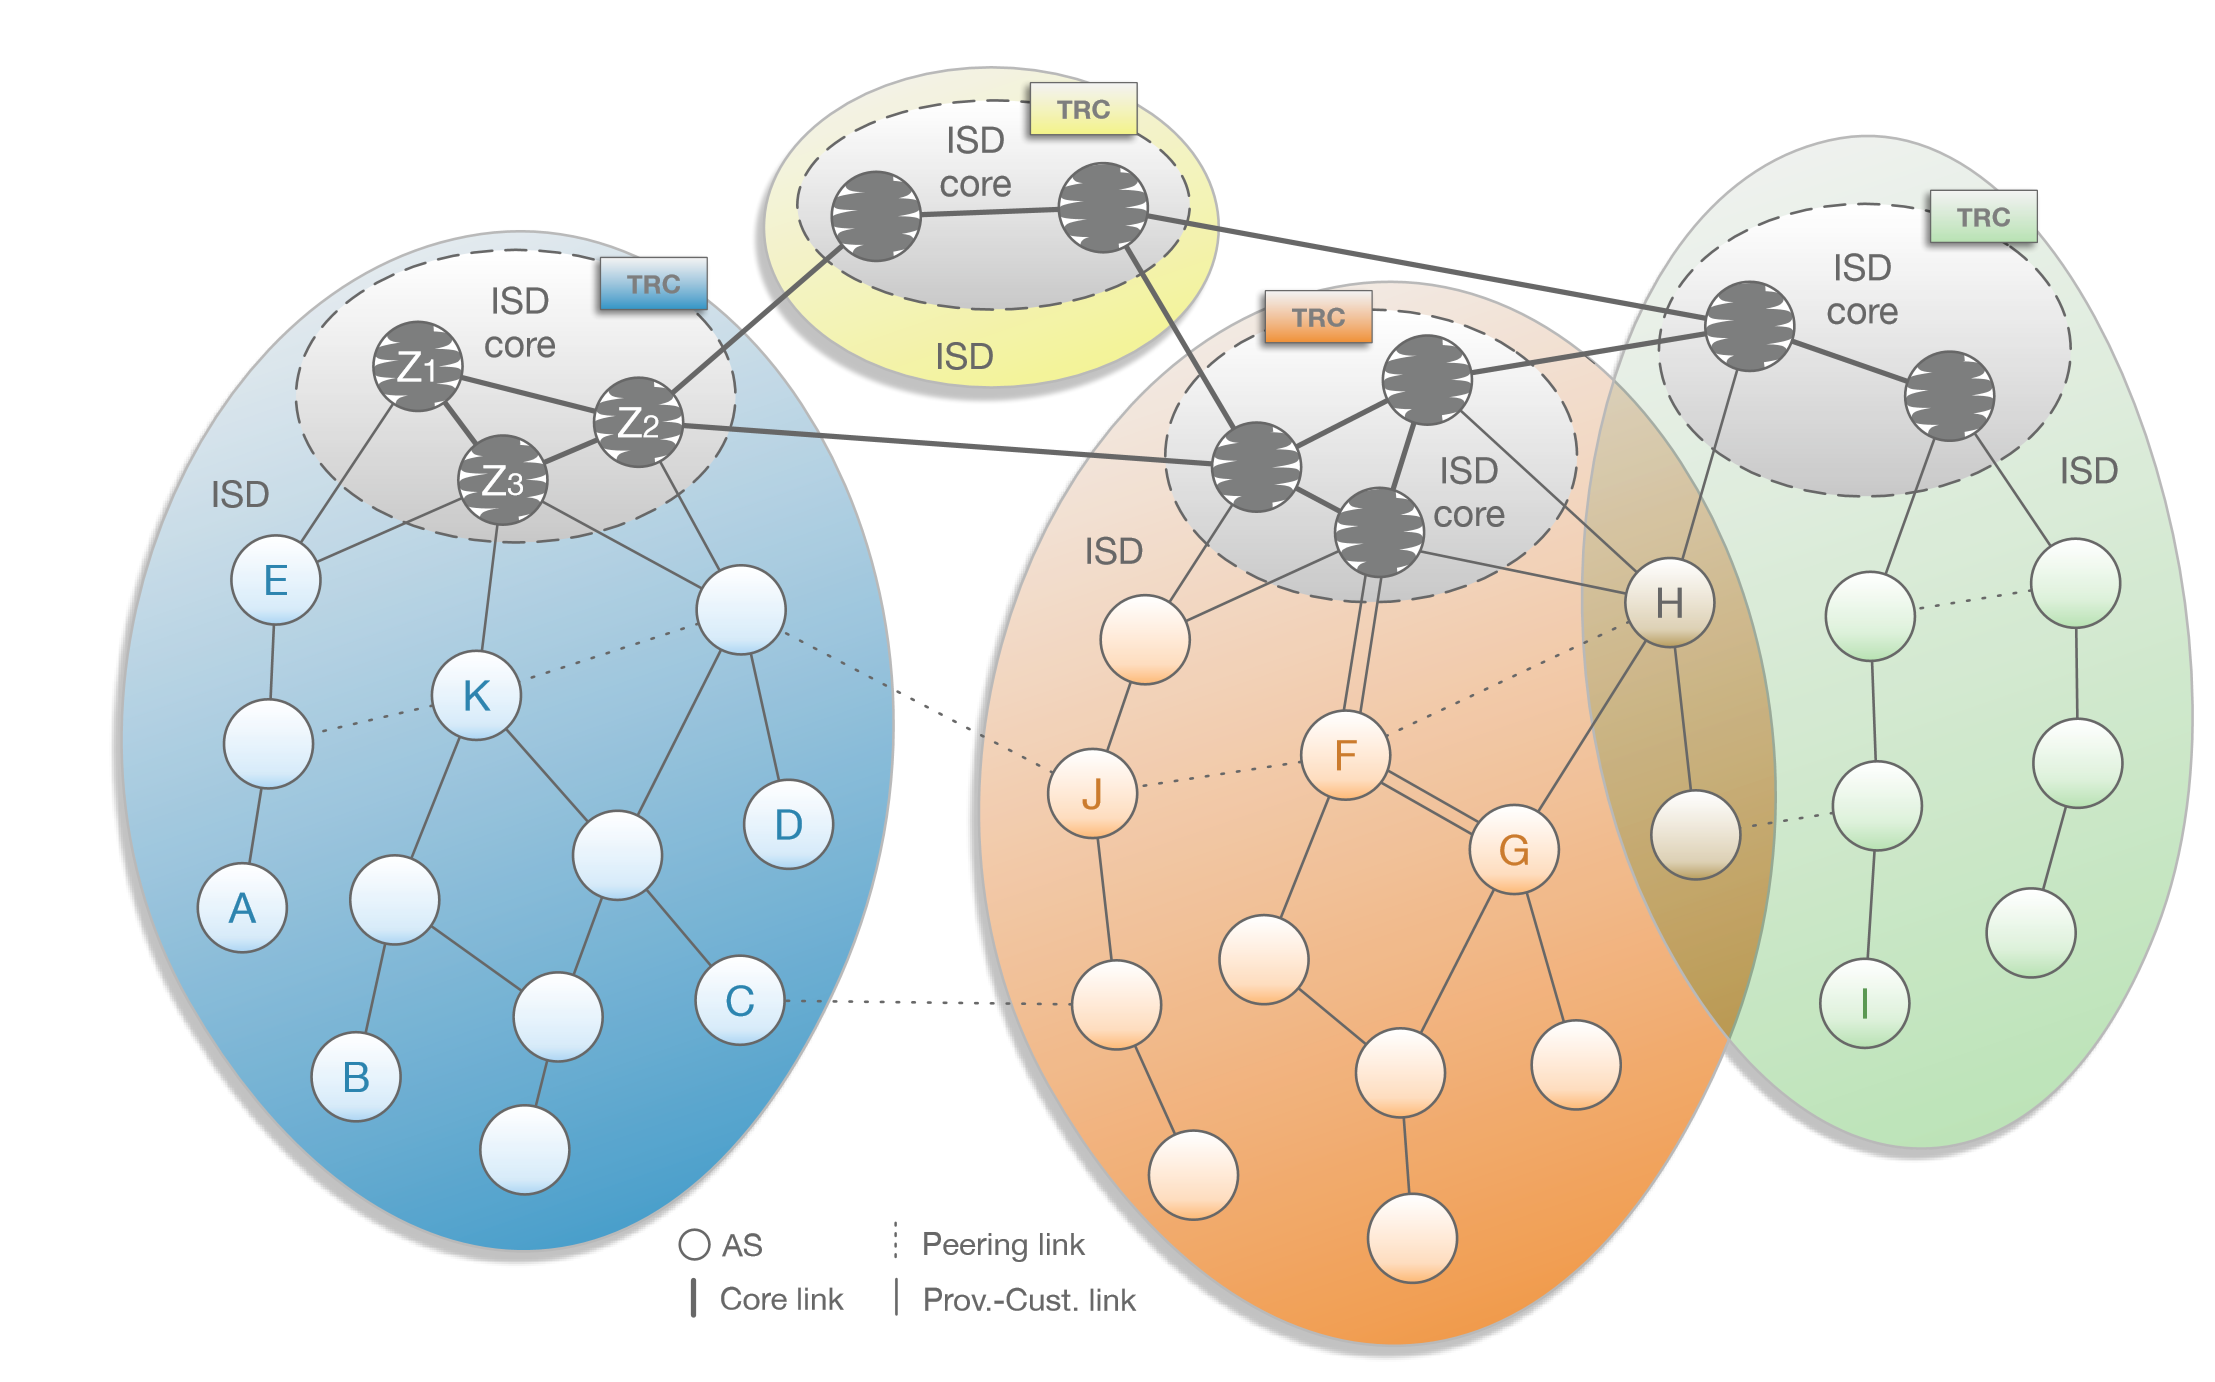
\includegraphics[width=\linewidth]{scion_overview.png}}
	\captionof{figure}{Schematic overview of a SCION network consisting of four ISDs \cite{scion_book}}
	\label{back:overview}
\end{figure}


\subsection{Network Structure}
\label{back:network_structure}
SCION organizes Autonomous Systems (ASes) into entities called Isolation Domains (ISDs). A selection of ASes in an ISD are designated 
core ASes responsible for administering the ISD. For example, the core ASes  negotiate the roots of trust used for authentication. An AS can join an ISD by connecting to an AS that already is a member of the ISD. Joining an ISD implies agreeing to the policies governing the ISD. \cite[Chapter~2]{scion_book}

\subsection{Isolation}
SCION divides the network into isolated entities called Isolation Domains and lets these ISDs manage their own part of the network, including the election of authorities and properties like routing policies and key agreement. This enables SCION to divide the control plane in a way such that one ISD is not influenced by changes in any other ISD. As an example, this mitigates outages (therefore increasing availability as desired) caused by accidentally or even maliciously misconfigured ASes, which make BGP announcements for addresses they have no control over. whereas In today's Internet, potentially every host could be affected. \cite[Chapter~3]{scion_book} Figure \ref{back:overview} shows a network with four ISDs, each consisting of multiple ASes.
	
\subsection{Path Selection}
SCION allows each host to control routes for outgoing and incoming packages. For each AS different paths, so called up-paths, are constructed using \textit{Path Construction Beacons} (PCBs). These PCBs reflect the constraints imposed by the ISD routing policy. ASes then announce over which of these paths they want to be reached. This technique, amongst other advantages, makes it possible to deploy effective mechanisms against Denial of Service attacks. Additionally, SCION offers a secure way of revoking failed paths and paths that do not conform to the route policy any more. \cite[Chapters~7, 10]{scion_book}
	
	\begin{figure}
		\centering
		\centerline{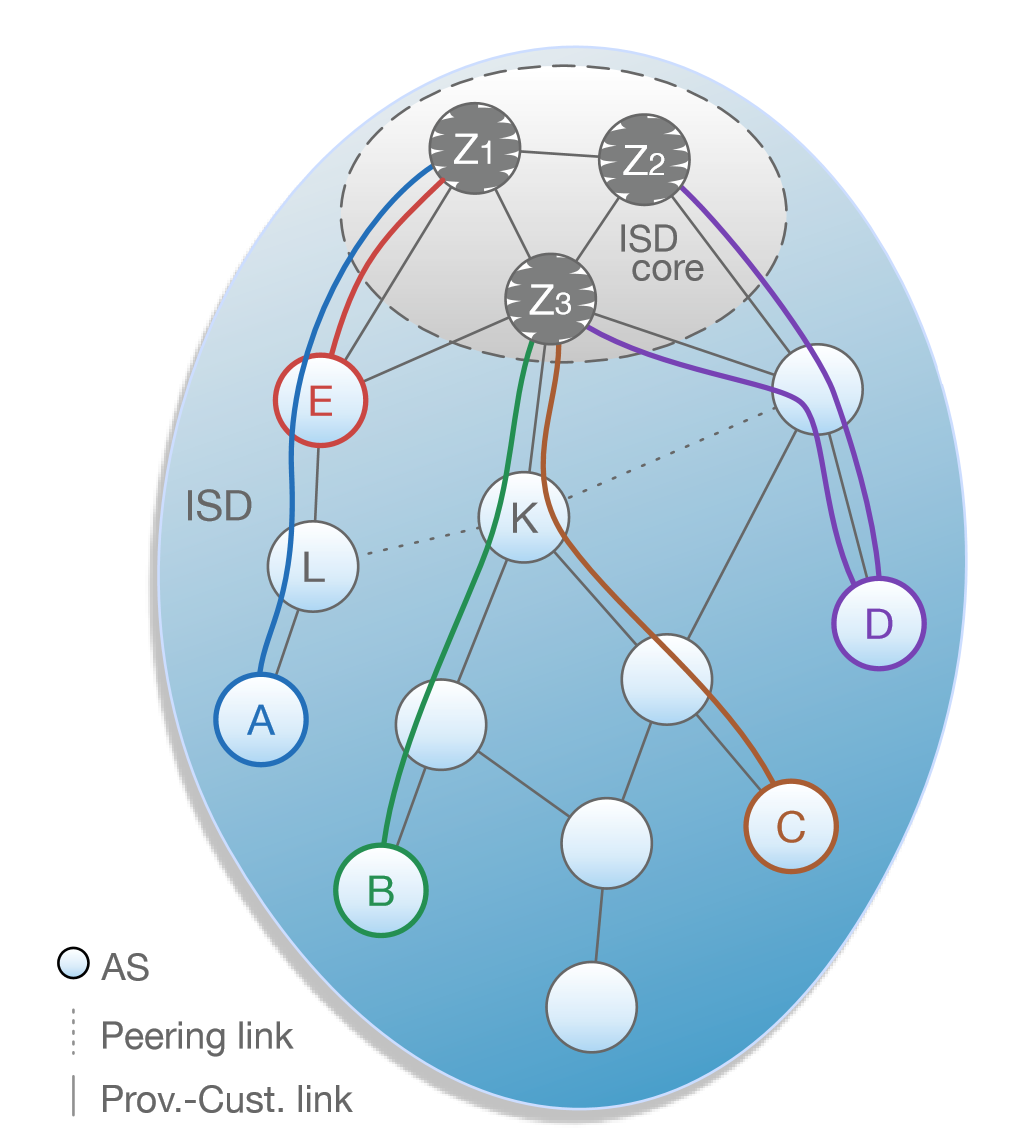
\includegraphics[height=8cm]{isd_paths.png}}
		\captionof{figure}{ISD with path segments for ASes A, B,C, D, and E \cite{scion_book}}
		\label{back:paths}
	\end{figure}

\subsection{Scalability}
The controlled path selection approach outlined above ensures great scalability, as opposed to source-based routing where every host needs to know the entire network topology. At the same time, the freedom of path selection is preserved. Furthermore, since routes are pre-determined, all the forwarding information is encoded in the package itself. This renders badly scaling routing and forwarding tables obsolete, all to the benefit of increased scalability. \cite{scion_book}


\section{SCION Architecture}

Following, important components of the SCION architecture are described. All the information is taken from \cite{scion_book}.
 
\subsection{Border Routers}
Border routers are responsible for inter-AS communication. They carry out packet forwarding based on the pre-determined path, encoded in each packet. Border routers work efficiently since the costly look up in a forwarding table is omitted.

\subsection{Beacon Servers}
The main function of the Beacon Server is to process path construction beacons (PCBs). The mechanism starts with a core AS generating initial PCBs and distributing them over the network. Beacon servers of non-core ASes upon receive propagate the PCBs down to their child ASes, such that the whole network is flooded. Through these beacons, ASes learn paths on which they can reach the ISD core. The AS then selects a subset of these paths and registers them using its Path server.

\subsection{Path Servers}
After processing PCBs, an AS registers at its local path server down-paths over which it wants to be reachable. This information is then used by other ASes to determine routes to that AS.

In reverse, the path server also functions as look up service via which an AS can retrieve path segments to reach another AS. When queried for an AS, the path server returns the paths available to reach the desired AS.

\subsection{Certificate Servers}
Local certificate servers manage and cache certificates of all members inside their AS, as well as the certificate issued by the ISD core to be used by the AS itself. For example, certificate servers support path servers by validating PCBs. \cite[Chapter~2]{scion_book}

A certificate server in the ISD core manages all certificates it handed out to ASes in its ISD and provides a validation service ASes can query.

\subsection{Name Servers}
Similar to the DNS system currently used in the Internet, name serves perform the translation from human-friendly names to addresses understood by SCION infrastructure. The path server is then queried to obtain end-to-end paths reaching the resolved address. \cite[Chapter~2]{scion_book} 


\section{SCION AS Management Framework}
\label{back:lmi}

For easy deployment and maintenance, SCION offers the SCION AS Management Framework which provides an intuitive web interface for deploying and managing ASes. The framework consists of a \lmi per AS and a global coordinator, the \lcs. This framework facilitates inter-AS communication by relaying connection requests between ASes. In Section \ref{back:network_structure} we explained how an AS can join an ISD by connecting to an AS that already is in said ISD. Such ISD join requests, for example, are handled by the framework. Figure \ref{back:deployment} shows three deployed ASes connected through the SCION AS Management Framework.

The following sections describe the two components of the framework in more detail.

\begin{figure}
	\centering
	\centerline{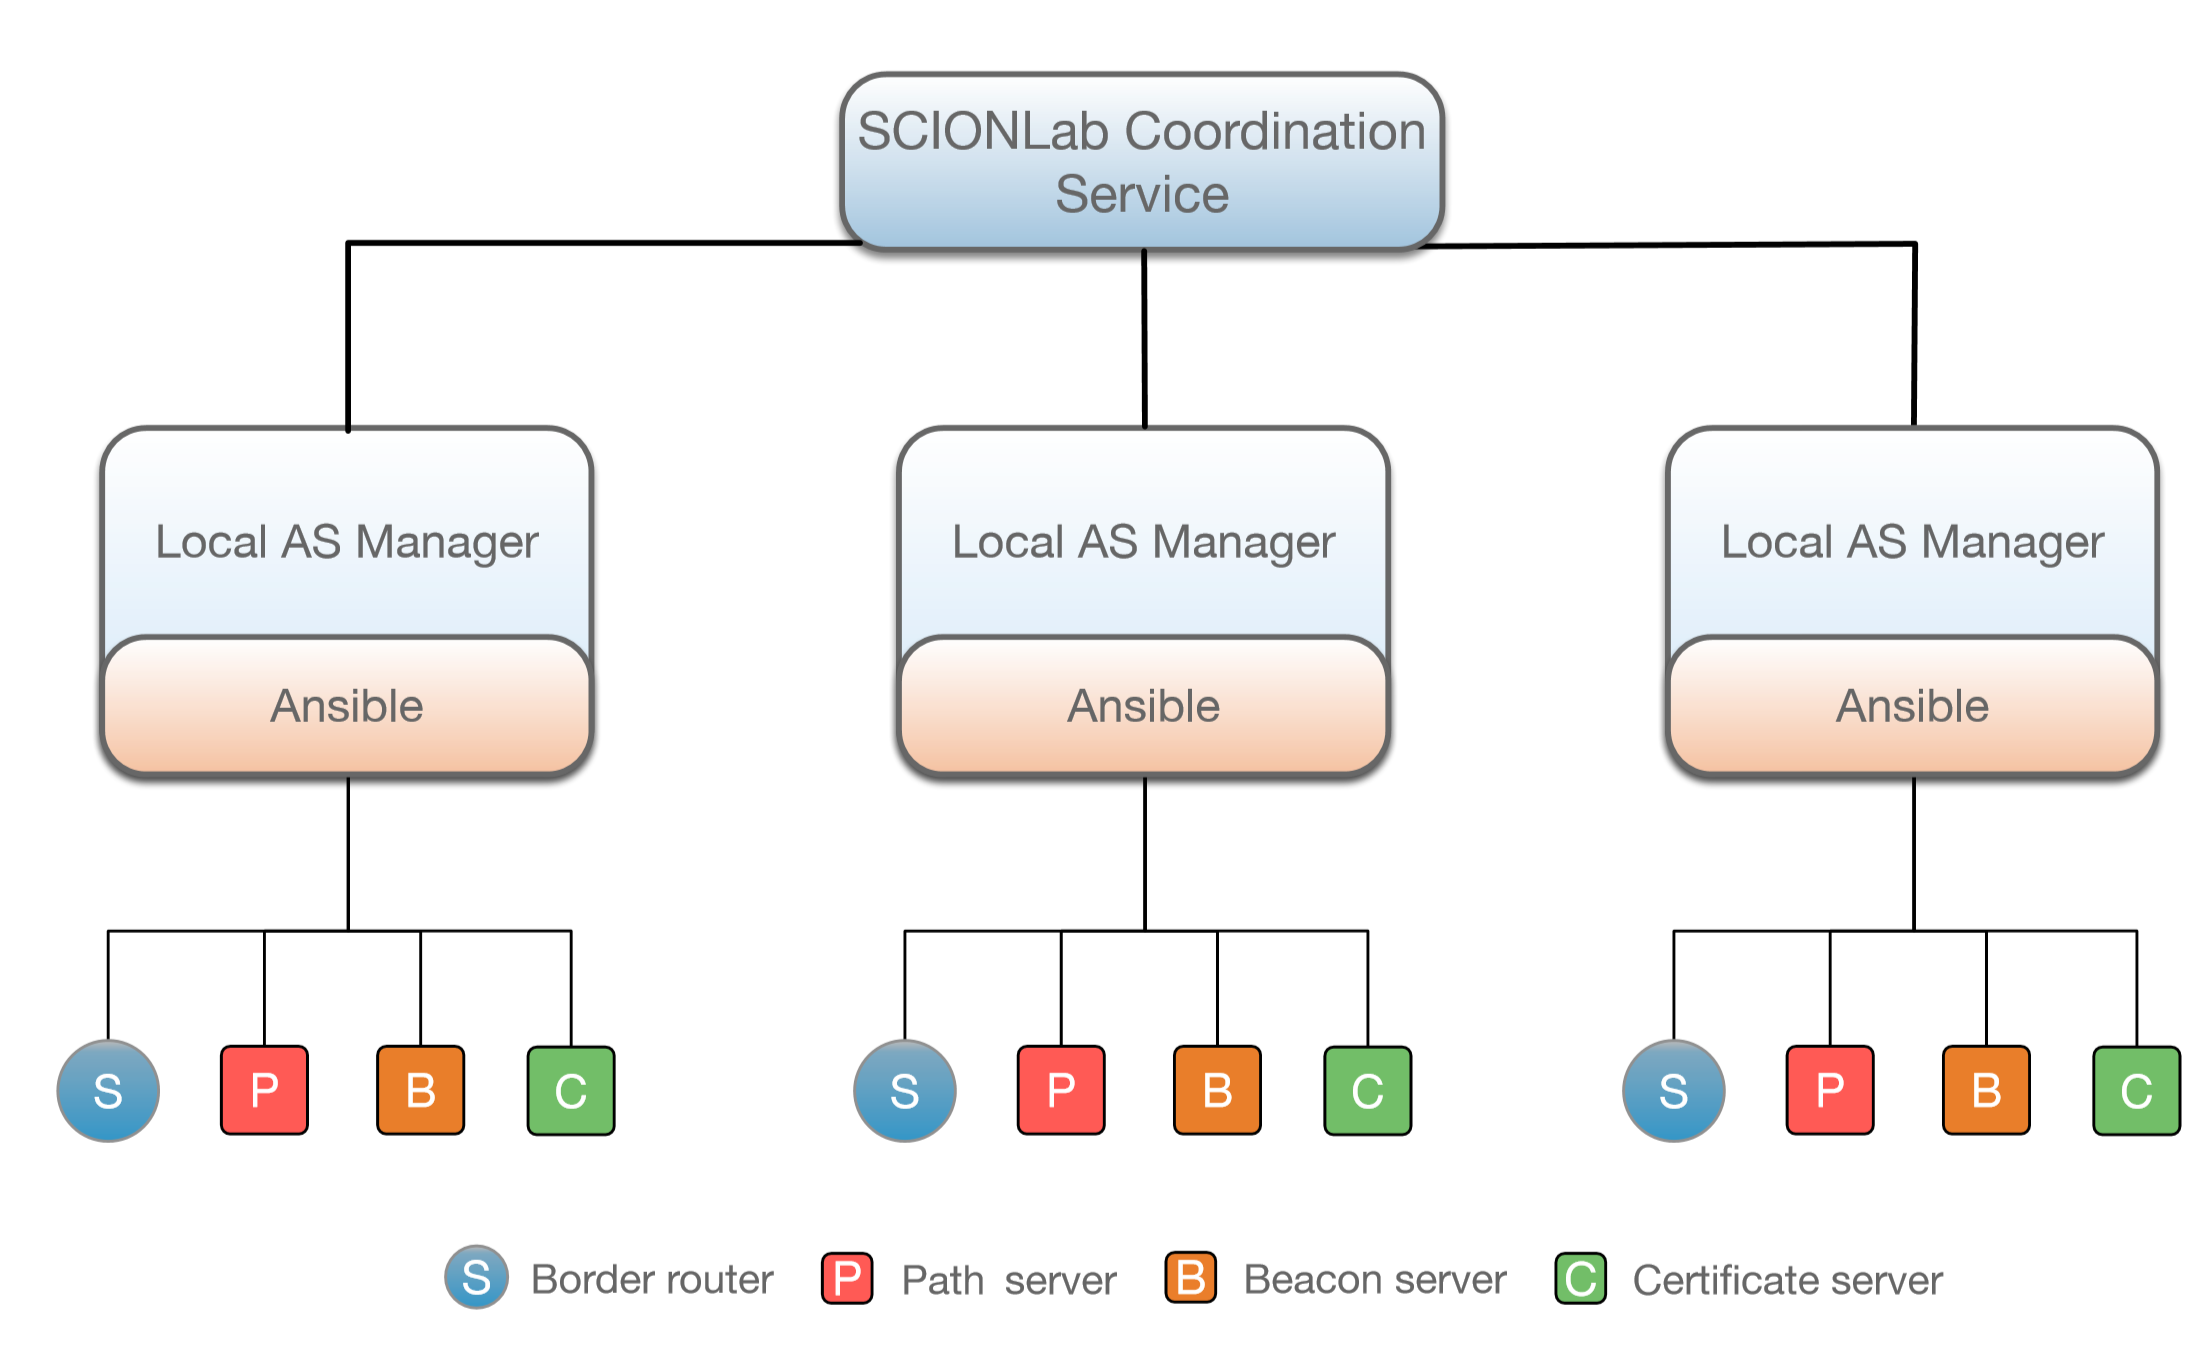
\includegraphics[width=\linewidth]{scion_deployment.png}}
	\captionof{figure}{Overview of deployment architecture showing the role of \lcs as mediator \cite{scion_book}}
	\label{back:deployment}
\end{figure}

\subsection{Local Management Service}

The \fnurl{\lmi}{https://github.com/netsec-ethz/scion-web} is the local component of the SCION AS Management Framework. It's run by the authority managing the AS, used to monitor and configure that AS. It offers a web interface through which, amongst other functionality, administrators can make connection requests to other ASes they wish to connect to. These requests, containing all the necessary data to set up a new link between the initiator and the remote AS, are then relayed via \lcs to the recipient AS. \cite[Chapter~10]{scion_book} In a similar fashion join requests for integrating an AS into an ISD can be issued using the \lmi. Other functionality involves generating the AS topology and the configurations to be deployed onto local servers.

Figure \ref{back:scionweb} shows the \lmi interface presented when making a connection request.

\begin{figure}
	\centering
	\centerline{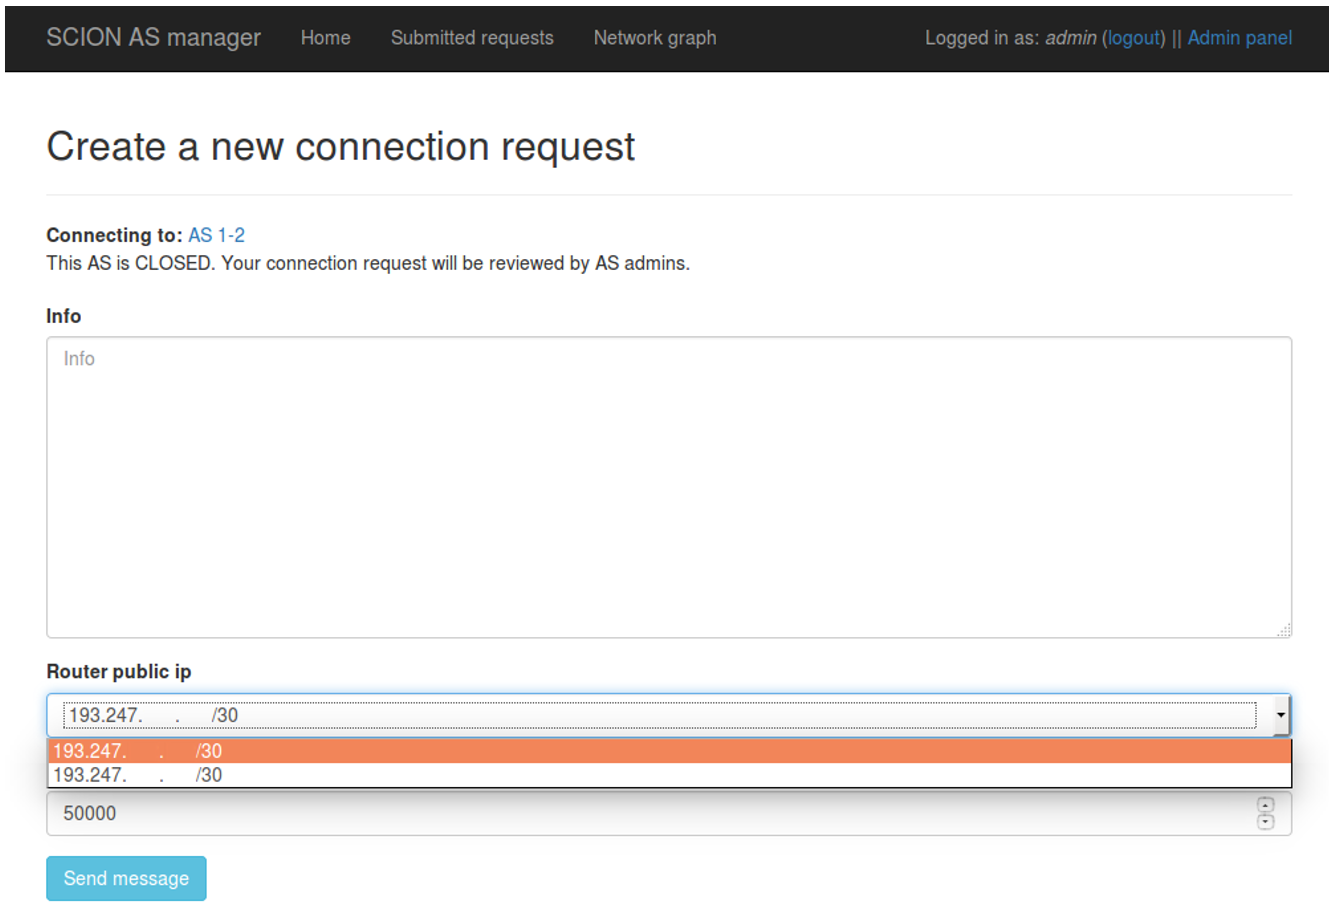
\includegraphics[width=\linewidth]{scionweb.png}}
	\captionof{figure}{\lmi used to make a connection request \cite{wirz}}
	\label{back:scionweb}
\end{figure}

\subsection{SCIONLab Coordination Service}
\label{back_scion_coord}

\fnurl{\lcs}{https://github.com/netsec-ethz/scion-coord} serves two purposes. For one it is part of the SCION AS Management Framework where it serves as a mediator between different \lmi instances. It provides information about available ISDs and ASes making it easy for new ASes to be created and connected to the SCION network. \lcs in the role of a mediator is not required by SCION. It's merely a tool to facilitate the deployment process in the early stages of adoption. Later, inter-AS connections will be negotiated between the involved parties directly. \cite[Chapter~10]{scion_book}

\lcs's second responsibility is the support of the \lee which lets interested organisations and institutions experiment with the unique capabilities of SCION. More detail about \lee and the role \lcs takes in it is available in Section \ref{back:scionlab}.

\section{SCIONLab Experimentation Environment}
\label{back:scionlab}

The \lee is a project started with the goal to provide a unique testbed environment, enabling researches to experiment with SCION and the features it offers. At the same time, it allows the SCION network to naturally grow by opening up the infrastructure. In SCIONLab, participants join by deploying their own ASes in the SCION network and then connecting to other SCIONLab ASes. Hence, SCIONLab forms a subset of the entirety of ASes deployed in the SCION network. Participants become an integral part of the network, actively partaking in routing. This allows researchers to conduct highly realistic experiments, not possible with other popular testbed environments. \cite[Chapter~10]{scion_book}

SCIONLab builds on the foundation of SCION AS Management Framework. It uses the same tools to offer a clean, easy-to-use way of joining the SCIONLab network.
As an example, \lcs facilitates the deployment of SCIONLab ASes for interested parties. It is envisioned to offer built in user administration capabilities, where users can register accounts and download SCIONLab configurations to be run on their hardware. Moreover, it also provides status updates about services running in the AS and notifications about new SCION versions. \cite[Chapter~10]{scion_book}

Summarized, the goals of \lee are:
\begin{itemize}
	\item Providing a unique testbed environment
	\item Opening up SCION to allow organic growth
	\item Allowing for realistic conduction of experiments
	\item Achieving above points with low overhead using user-friendly tools such as the \lcs
\end{itemize}

Figure \ref{scionlab_figure} shows an example of an envisioned SCIONLab environment.

\begin{figure}
	\centering
	\centerline{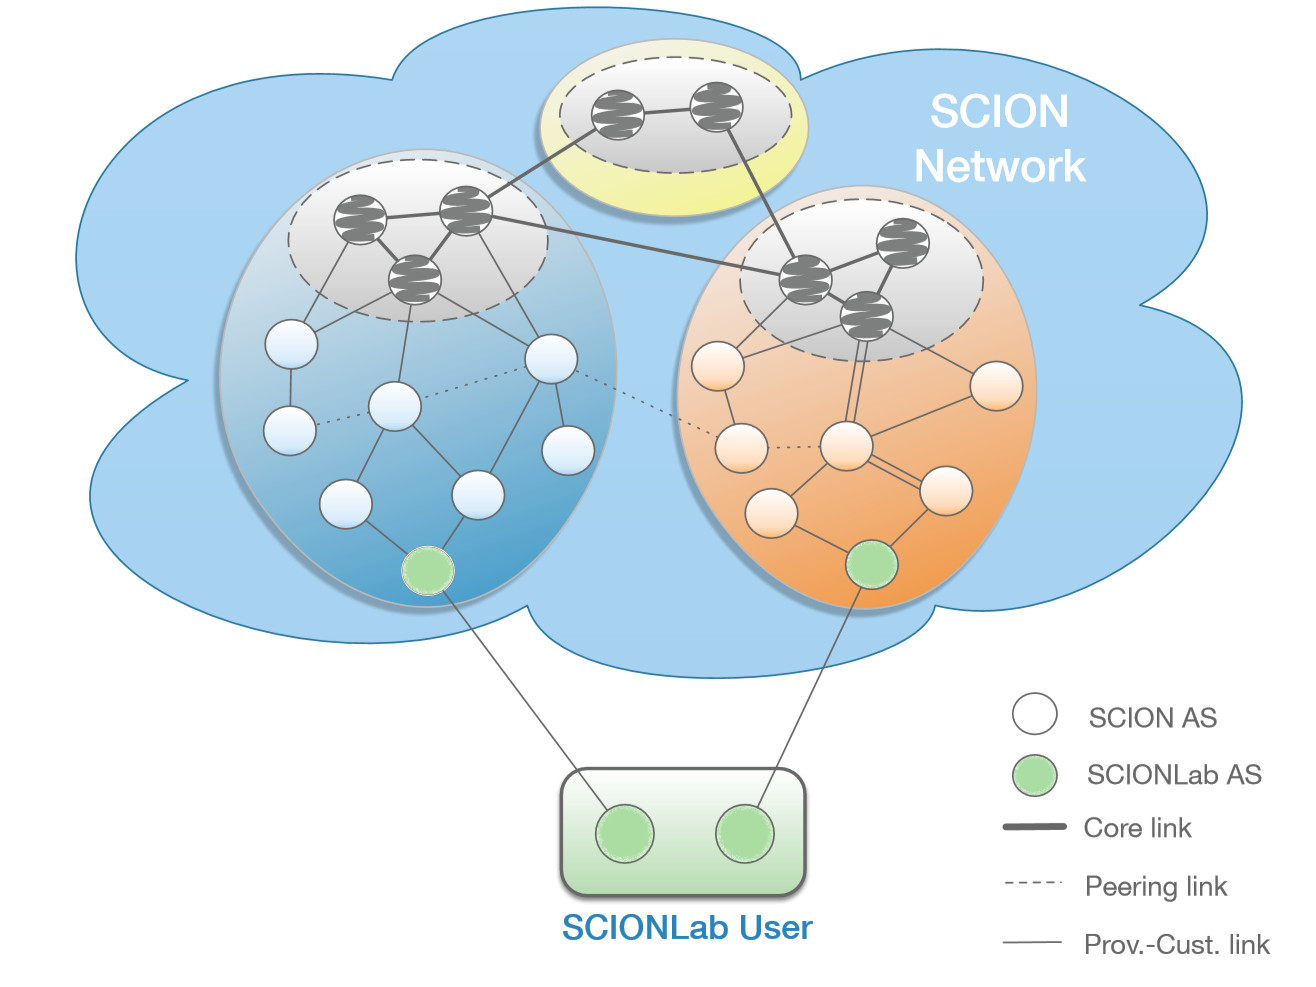
\includegraphics[width=\linewidth]{scionlab.png}}
	\captionof{figure}{An envisioned SCIONLab  testbed environment \cite{scion_book}}
	\label{scionlab_figure}
\end{figure} % Background Theory 
\chapter{Related Work}

The following sections provide a brief overview of other testbed environments for running network and distributed systems experiments. In particular, their approach of organising and managing network nodes and their way of handling users enrolled in experiments is highlighted.

\section{PlanetLab}

\fnurl{PlanetLab}{https://www.planet-lab.org/} is an open platform for computer networking and distributed systems research. It allows the deployment and testing of newly developed network protocols, distributed algorithms, peer-to-peer software and \fnote{CDNs}{Content Delivery Networks}. \cite{MA} For conducting tests, each project has access to a set of globally distributed virtual machines. These sets, called slices in PlanetLab terminology, run on physical nodes provided and maintained by users of PlanetLab, mainly research institutions.

\subsection{PlanetLab Node Management}

For an institution to be granted access to PlanetLab, it has to add its own computational resources to the PlanetLab network. \cite{planetlab_two_nodes} These nodes are remotely managed by PlanetLab operational staff. Local administrators are not given root access and are merely allowed to modify certain parameters, such as outgoing network bandwidth. \cite{planetlab_hosting_req} A Principal Investigator (PI) at each site is responsible for approving accounts and assigning them to slices. Furthermore, the PI locally enforces the PlanetLab Acceptable Use Policy (AUP). After instantiating a slice, users are given \fnote{SSH}{Secure Shell} access with root privileges to nodes in their slice. However, this root access is restricted as it does not allow changes to hardware and network configurations. \cite{planetlab_user_guide} 

Comparing to \lee, there are some fundamental differences:

\begin{itemize}
	\item In \lee, each project joins with its own resources. Neither are there restrictions regarding system configuration, nor are nodes managed by SCIONLab operational staff.
	\item There is no assignment to slices by a PI in SCIONLab. The deployment of nodes in SCIONLab is left entirely to the project team.
	\item Deployed nodes do not necessarily need to be virtualized. There are configurations for running SCION directly on physical machines.
	\item Since there are no PIs in SCIONLab, the intermediate step of creating accounts via PI is omitted. Institutions directly register their accounts via \lcs.
	\item SCIONLab uses a novel approach of pre-authenticated accounts with pre-established connections to get research institutions aboard. This allows invited parties to start using SCIONLab with minimal overhead.
	\item Developed from ground up with simplicity in mind, the \lee offers easy-to-use node management tools.
\end{itemize}

\section{GENI}

Similar to PlanetLab, \fnurl{GENI}{http://www.geni.net/} (Global Environment for Network Innovations) is a testbed environment designed for networking and distributed systems research. Like PlanetLab, GENI uses the notion of slices to describe a set of geographically distributed virtual and physical hosts, instantiated for an experiment. The unique feature of GENI is its "deep programmability" capability which lets users connect compute resources on the link layer and replace above layers with custom protocols. \cite{geni}

In GENI, each project is led by a single individual; the project lead. The project lead is responsible for allocating slices and assigning project members to them. Slices consist of different resource providers available in the GENI network, so called aggregates.

Aggregates are hosted by institutions and managed by local operators. In order to start using GENI, an account must be registered. However, thanks to tight collaboration with many institutions, the institutions account may be used to register for GENI. Additionally, since experiments on GENI often revolve around new services, GENI allows end users, who are not affiliated with the project, to opt in, in order to bring real traffic to experiments. \cite{geni}


\section{Fed4FIRE}

\fnurl{FED4FIRE}{https://www.fed4fire.eu/} strives for creating a large federation of experimentation facilities and network testbeds in Europe. The main idea behind this initiative is to simplify the use of already existing testbed environments, thus making it possible for researchers to collaborate by sharing existing test facilities in the broad field of \fnote{ICT}{Information and Communication Technology}. This also allows researchers to use multiple testbeds for their experiments. \cite{fire_book}

FED4FIRE offers its facilities in two ways: Open Calls are selected projects which receive financial support to be carried out. The other possibility, Open Access, allows every interested party to run their projects, without being funded.

Accounts are registered at a FED4FIRE authority and then used to create new projects, similar to PlanetLab and GENI. The architecture consists of multiple testbed environments, all aggregated under the FED4FIRE initiative. By the nature of this very heterogeneous design, the management of the environment is much more complicated than in SCIONLab. \cite{fire_book} % Discussion of Related Work
\chapter{Requirements Engineering}
\label{req}


With the introduction of SCIONLab, \lcs now plays a significant role in the \lee. Because of this, a set of new requirements arose, focusing on making the service an intuitive, user friendly tool, while at the same time increasing the robustness of the system. This shift from a mediator to an online account management tool, allowing users to register accounts and download their SCION configurations in order join the network with minimal overhead, demands an extension of initial requirements.

\section{Functional Requirements}
\label{func_req}

To make \lcs meet the functionality outlined above, the following requirements were gathered:

\begin{enumerate}  
	\item \textit{A mechanism to verify users' email addresses:}\\
		This increases the authenticity of registered accounts. This also ensures that users can be contacted by email.
	\item \textit{A mechanism to manually activate users who signed up successfully:}\\
		Not all users should immediately be granted access to \lcs. Administrators need to be able to audit registration requests.
	\item \textit{A mechanism to protect the service against automated account creation:}\\
		This safety measurement protects the service from spam and the creation of fake accounts.
	\item \textit{New functionality is validated using CircleCI's testing environment:}\\
		This increases development productivity and ensures new additions do not break \lcs.
	\item \textit{A fast and easy way to deploy the service onto multiple machines:}\\
		Since \lcs is evolving quickly, it is required that it can be deployed onto the target machine effortlessly.
	\item \textit{A system for sending notifications to users:}\\
		Users should be notified if the status of their ASes change or when new versions of SCION are available.
	\item \textit{Implementation of missing APIs between \cords and the \lmi:}\\
		This ensures flawless operation of \lcs in its role as mediator.
	\item \textit{A visualization of the SCIONLab Experimentation network accessible by users:}\\
		This makes it easy for new users to get an overview of the SCIONLab network and helps them join an ISD.
\end{enumerate}

\section{Non-Functional Requirements}
\label{non-func_req}

Non-Functional requirements comprise the following points:

\begin{enumerate}
	\item \lcs aims to be an easy to use tool.
	\item None of its functionality should require the user to invest a great amount of work.
	\item It is preferred to hide as much complexity as possible from users.
	\item The web interface of the service is required to be fast, clean and responsive, since it will be amongst the first impressions users get of SCION.
	\item The web interface needs to be visually appealing, both on desktop and mobile devices.
	\item In terms of maintainability, \lcs aims for easy extensibility as the project evolves fast and new requirements need to be integrated with minimal effort.
\end{enumerate} % Design Objectives
\chapter{Architecture Overview}

\section{Design Overview}

Figure \ref{archi:overview} shows an overview of the architectural design of \lcs. All the components and services are described in detail in the following sections.

\begin{figure}
	\centering
	\centerline{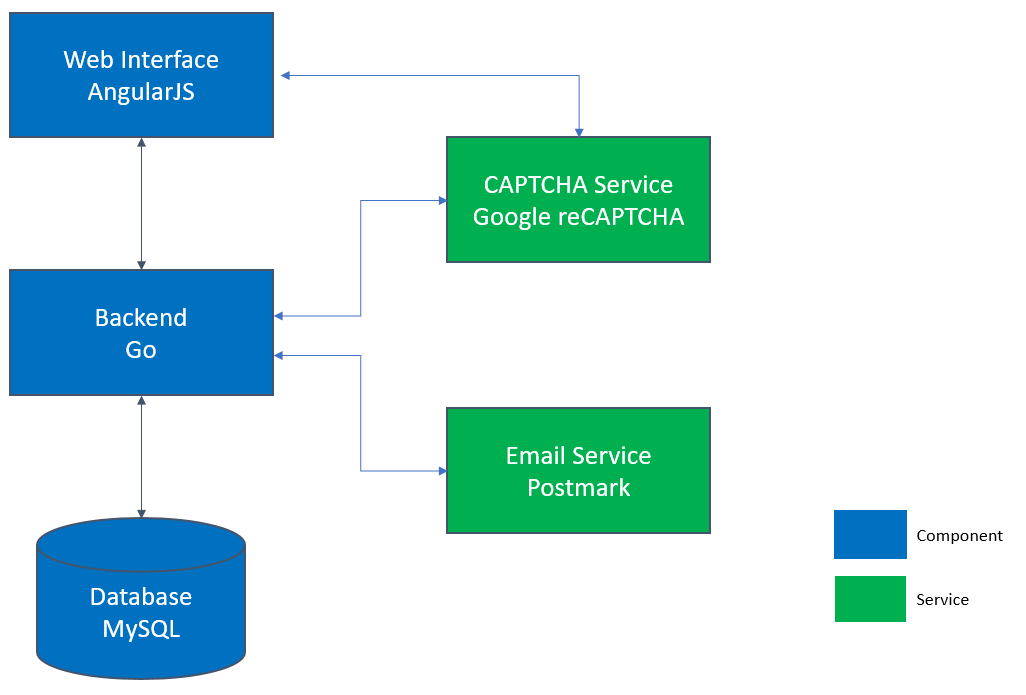
\includegraphics[width=\linewidth]{architecture_overview_new.png}}
	\captionof{figure}{Schematic overview of \lcs architecture, showing its components and the services it uses}
	\label{archi:overview}
\end{figure}

\section{Components}
In the following sections, component denotes a part that directly belongs to the \lcs architecture.

\subsection{Database}

\lcs uses a MySQL database as storage system. MySQL is one of the most widely used relational database management systems. In this project a free to use, open-source version is used. It stores basic entities such as users, their corresponding accounts, ASes deployed by users and connection requests sent between ASes. If a user makes use of a virtual machine to run SCION, configurations for this set up are stored as well. Another purpose is to keep track of the state aforementioned entities are in. It directly interfaces with the back end web server which is the only component it receives queries from.

\subsection{Back End Server}

The centre piece of the \lcs is the back end server. It interfaces with all the other components via a set of well defined APIs, therefore functioning as a mediator. It provides the following functionality:

\begin{itemize}
	\item Serving web pages to the \lcs web interface
	\item Processing of API calls received from the \lcs web interface
	\item Processing of API calls received from SCION \lmi
	\item Controlling access to resources
	\item Preparing emails and handing them over to Postmark servers for sending
	\item Processing and manipulating data retrieved from the database
\end{itemize}

\subsection{Web Interface}

The web interface is the front end part of the \lcs. It is the graphical interface between users and the system. It closely interacts with the back end server, to which it makes API calls and from which it receives all required data. The following functionality is offered by this component:

 \begin{itemize}
 	\item Ability to register new users
 	\item Login for existing users
 	\item A personal page per user showing account details and allowing to download a SCIONLab VM image
 	\item An administrator panel for managing pending user registrations
 	\item A landing page for users, successfully verifying their email address

 \end{itemize}

\section{Services}

\lcs makes use of multiple services to outsource certain tasks. These services are described in the subsections that follow.

\subsection{Postmark}
\label{archi:postmark}

\lcs uses \fnurl{Postmark}{https://postmarkapp.com/} for email sending. An early requirement was to use a local \fnote{MTA}{Mail Transfer Agent - The software running on an email server}. However, as outlined in Section \ref{impl_email_package}, this proved to be very unreliable. The decision was then to switch to an external provider that handles the complexity. Postmark guarantees fast and reliable delivery of all transactional emails sent by \lcs. \cite{postmark}

\subsection{Google reCAPTCHA}
As a measurement against bots that create fake SCIONLab accounts the web interface of \lcs contains a \fnote{CAPTCHA}{Completely Automated Public Turing test to tell Computers and Humans Apart} widget which needs to be solved in order to create an account. \lcs makes use of the Google reCAPTCHA service for implementing this functionality.

\section{Continuous Integration}
\label{archi:ci}

\fnurl{CircleCI}{https://circleci.com/} is a continuous integration utility that, once set up for a project, automatically runs unit tests for newly added code using cloud technologies. The feedback produced includes a comprehensive list of all tests it ran, showing which tests failed and for what reasons. This enables the \lcs development team to validate pull requests before they are merged into the master branch. CircleCI tightly ties into \fnurl{GitHub}{https://github.com/}, showing the outcome of the test suite directly on the pull request page.

 Additionally, new code is reviewed using \fnurl{Reviewable}{https://reviewable.io}. Reviewable keeps track of changes, as pull requests evolve with new commits. To be merged, all tests on CircleCI must pass and all discussions on Reviewable must be resolved.


\section{Deployment}
\label{archi:ansi}

Manually setting up a \lcs instance on a remote machine requires many steps. Hence, doing it often  and for multiple machines very quickly becomes a cumbersome task. To automate this process we use \fnurl{Ansible}{https://www.ansible.com/}. Ansible is an agentless IT automation engine with the goal to end repetitive tasks. It modifies a system in such a way that it matches the state described in configuration files, the playbooks. This makes the deployment, if the playbook is written carefully, idempotent.












 % Feature Design
\chapter{Implementation}
\label{impl}

The following sections contain in-depth descriptions of the design and implementation process of major additions developed throughout this thesis. Less extensive improvements, addressing the security and maintainability of \lcs, are described in appendix \ref{misc}.

\section{Initial State}

At the start of this thesis, a basic version of \lcs had already been implemented. The implementation consisted of the back end server written in \fnurl{Go}{https://golang.org/}, the web interface implemented in \fnurl{AngularJS}{https://angularjs.org/} and the \fnurl{MySQL}{https://www.mysql.com} database. While operational, \lcs was lacking desired functionality. Relevant for this thesis were particularly the weak user registration process, which did not perform any checks to ensure validity of submitted data. When logging in, users were presented with a simple page, merely showing credentials needed to connect to SCIONLab. It was not possible to download configurations and virtual machine images for running SCION. Furthermore, \lcs had no way of communicating with users via email.


This basic implementation was enhanced with new functionality as described in the rest of this chapter.

\section{Email Address Verification}
\label{impl_email_veri}

Two options were evaluated for email verification. Email callback verification and verification based on email exchange.

Email callback verification finds its use mostly as anti-spam measure in \fnote{SMTP}{Simple Mail Transfer Protocol} servers. The verification is carried out in the same way as sending an email to the target email address. However, instead of following through and sending actual email content, the process is aborted as soon as the remote mail exchanger accepts or rejects the recipient address as invalid. The response is the same \code{OK} or \code{Unknown user} as when running the protocol with the intent to send an email. \cite{callback_verification}
Email callback verification, however, suffers from unreliability \cite{callback_verification} which makes it not suitable for \lcs.

Instead, a robust approach based on email exchange was chosen. Upon registration users receive a link with a unique identifier. When they follow the link this is registered by the system and the users' email addresses are marked as verified. Figure \ref{veri:dia} shows a message sequence diagram of the process implemented.

\begin{figure}
	\centering
	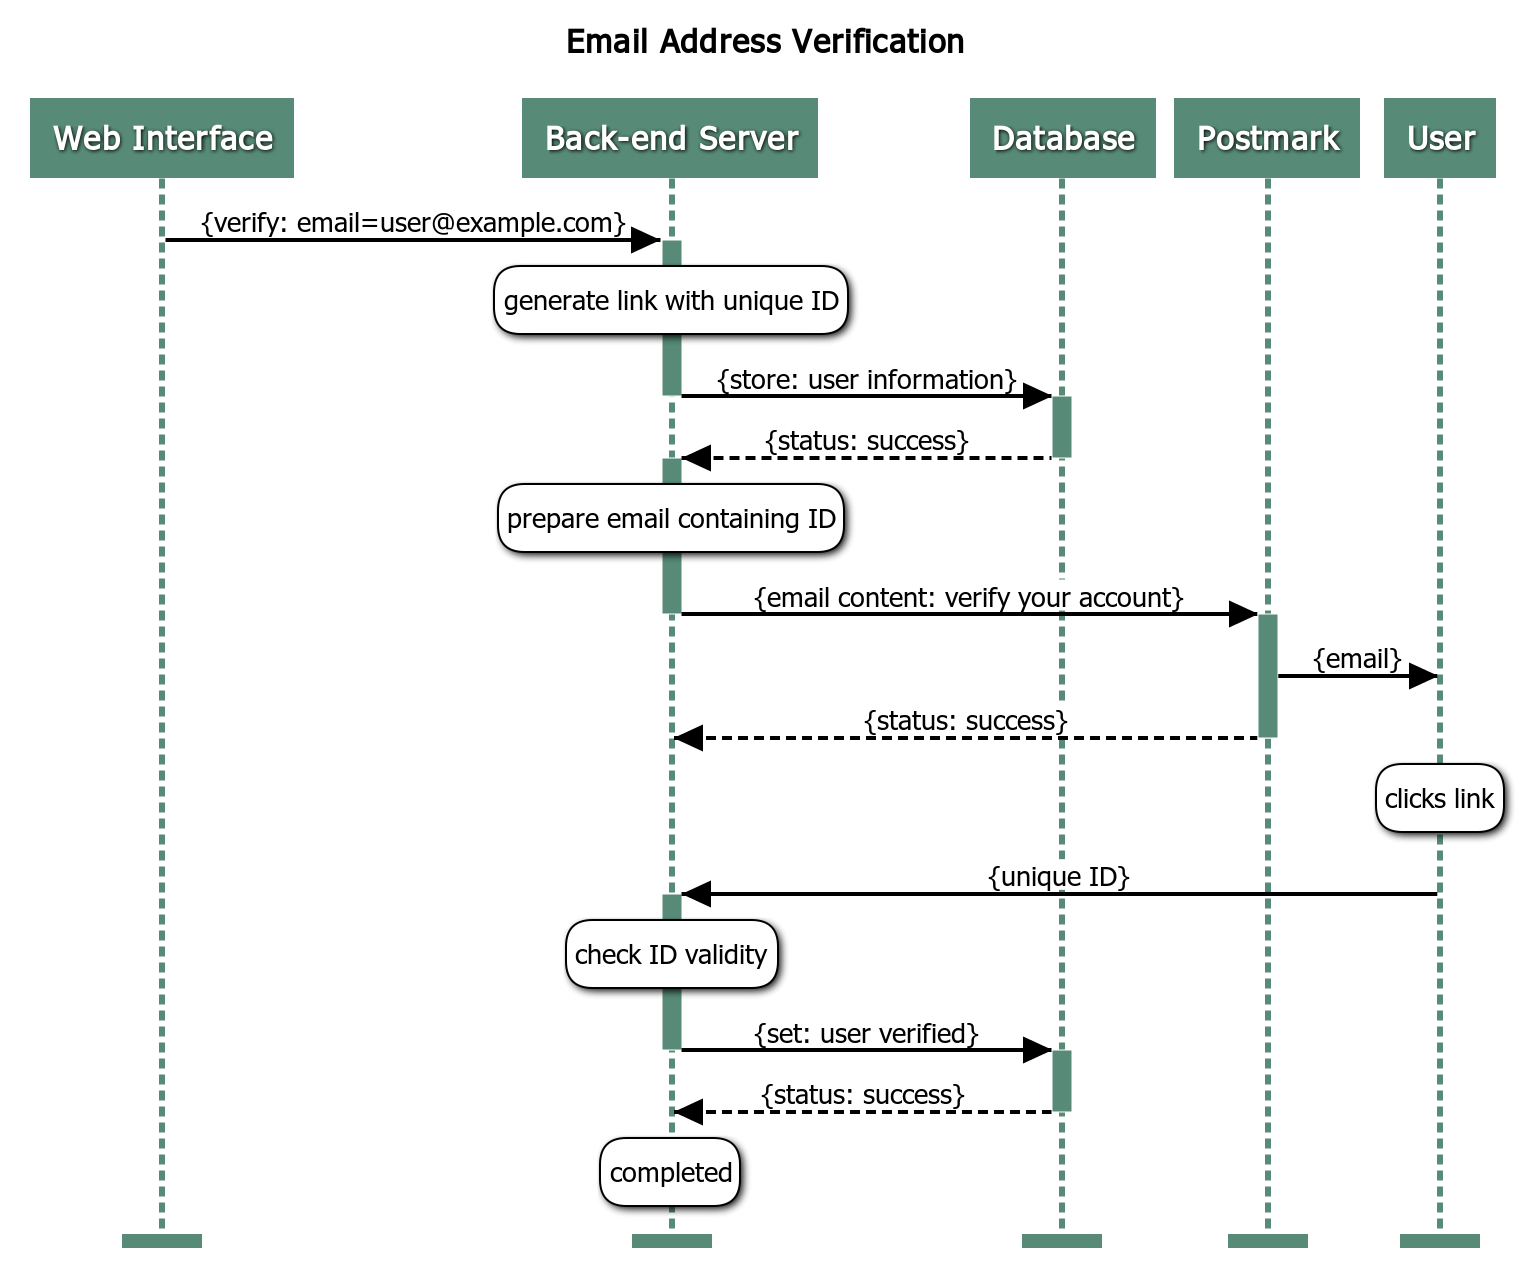
\includegraphics[width=\linewidth]{email_verification.png}
	\captionof{figure}{Sequence diagram showing the messages exchanged for the Email Verification feature}
	\label{veri:dia}
\end{figure}

\subsection{Email package}
\label{impl_email_package}

As already mentioned in Section \ref{archi:postmark}, the initial requirement was to support a local SMTP server for sending emails. Since \lcs originally did not have the ability to send emails, a new, self-written email package was added to the back end server. It was communicating with an \fnote{Exim}{Exim is a popular MTA for UNIX based systems} instance running on the same server. Extensive testing showed that the approach of supporting and maintaining a local MTA is too complex to implement in a reliable fashion for this project. While tweaking the email headers and content was sufficient for the email not to be marked as spam by \fnoteurl{SpamAssassin}{http://spamassassin.apache.org/}{A sophisticated spam filter} (see Figure \ref{exim_spam}), missing \fnote{MX Records}{Mail Exchange Resource Record - A record specifying a mail server in the DNS system} and absent \fnote{DKIM}{DomainKeys Identified Mail - a method to detect email spoofing} authentication (see Figure \ref{exim_auth}) often caused emails to not reach the inbox of users. It was then decided to outsource this complexity to Postmark, as described in Section \ref{archi:postmark}. As a result, the email package was changed to make use of Postmark's APIs, instead of interfacing with the local MTA. The outcome of the same spam detection and authentication tests ran with Postmark as mail provider are shown in Figures \ref{postmark_spam} and \ref{postmark_auth}.

\begin{figure}
	\centering
	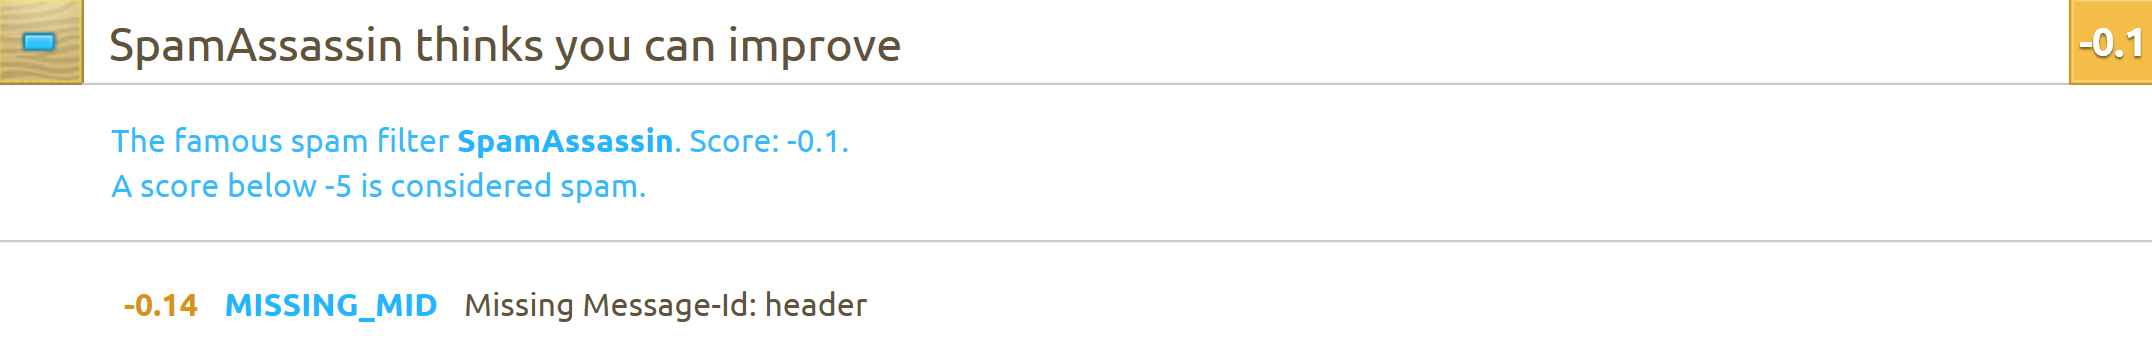
\includegraphics[width=\linewidth]{exim_spamassassin.png}
	\captionof{figure}{Result of SpamAssassin ran against local Exim SMTP server (Run on \href{https://www.mail-tester.com/}{Mail-Tester})}
	\label{exim_spam}
\end{figure}

\begin{figure}
	\centering
	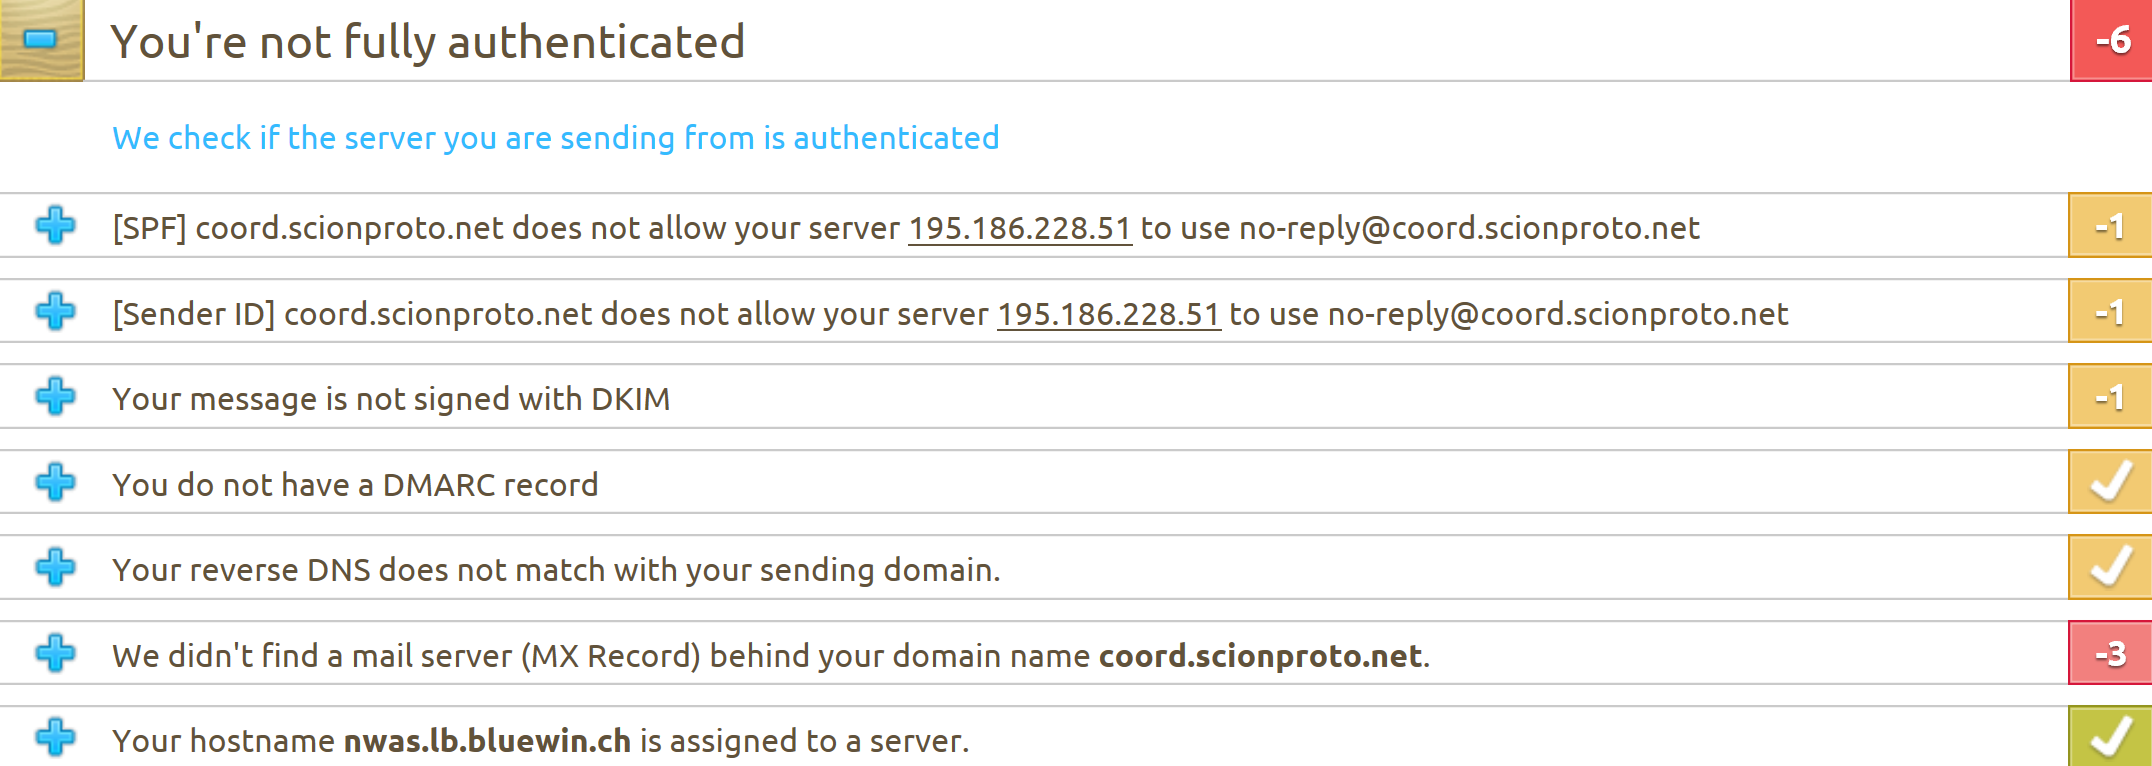
\includegraphics[width=\linewidth]{exim_auth.png}
	\captionof{figure}{Authentication report for the local Exim SMTP server (Run on \href{https://www.mail-tester.com/}{Mail-Tester})}
	\label{exim_auth}
\end{figure}

\begin{figure}
	\centering
	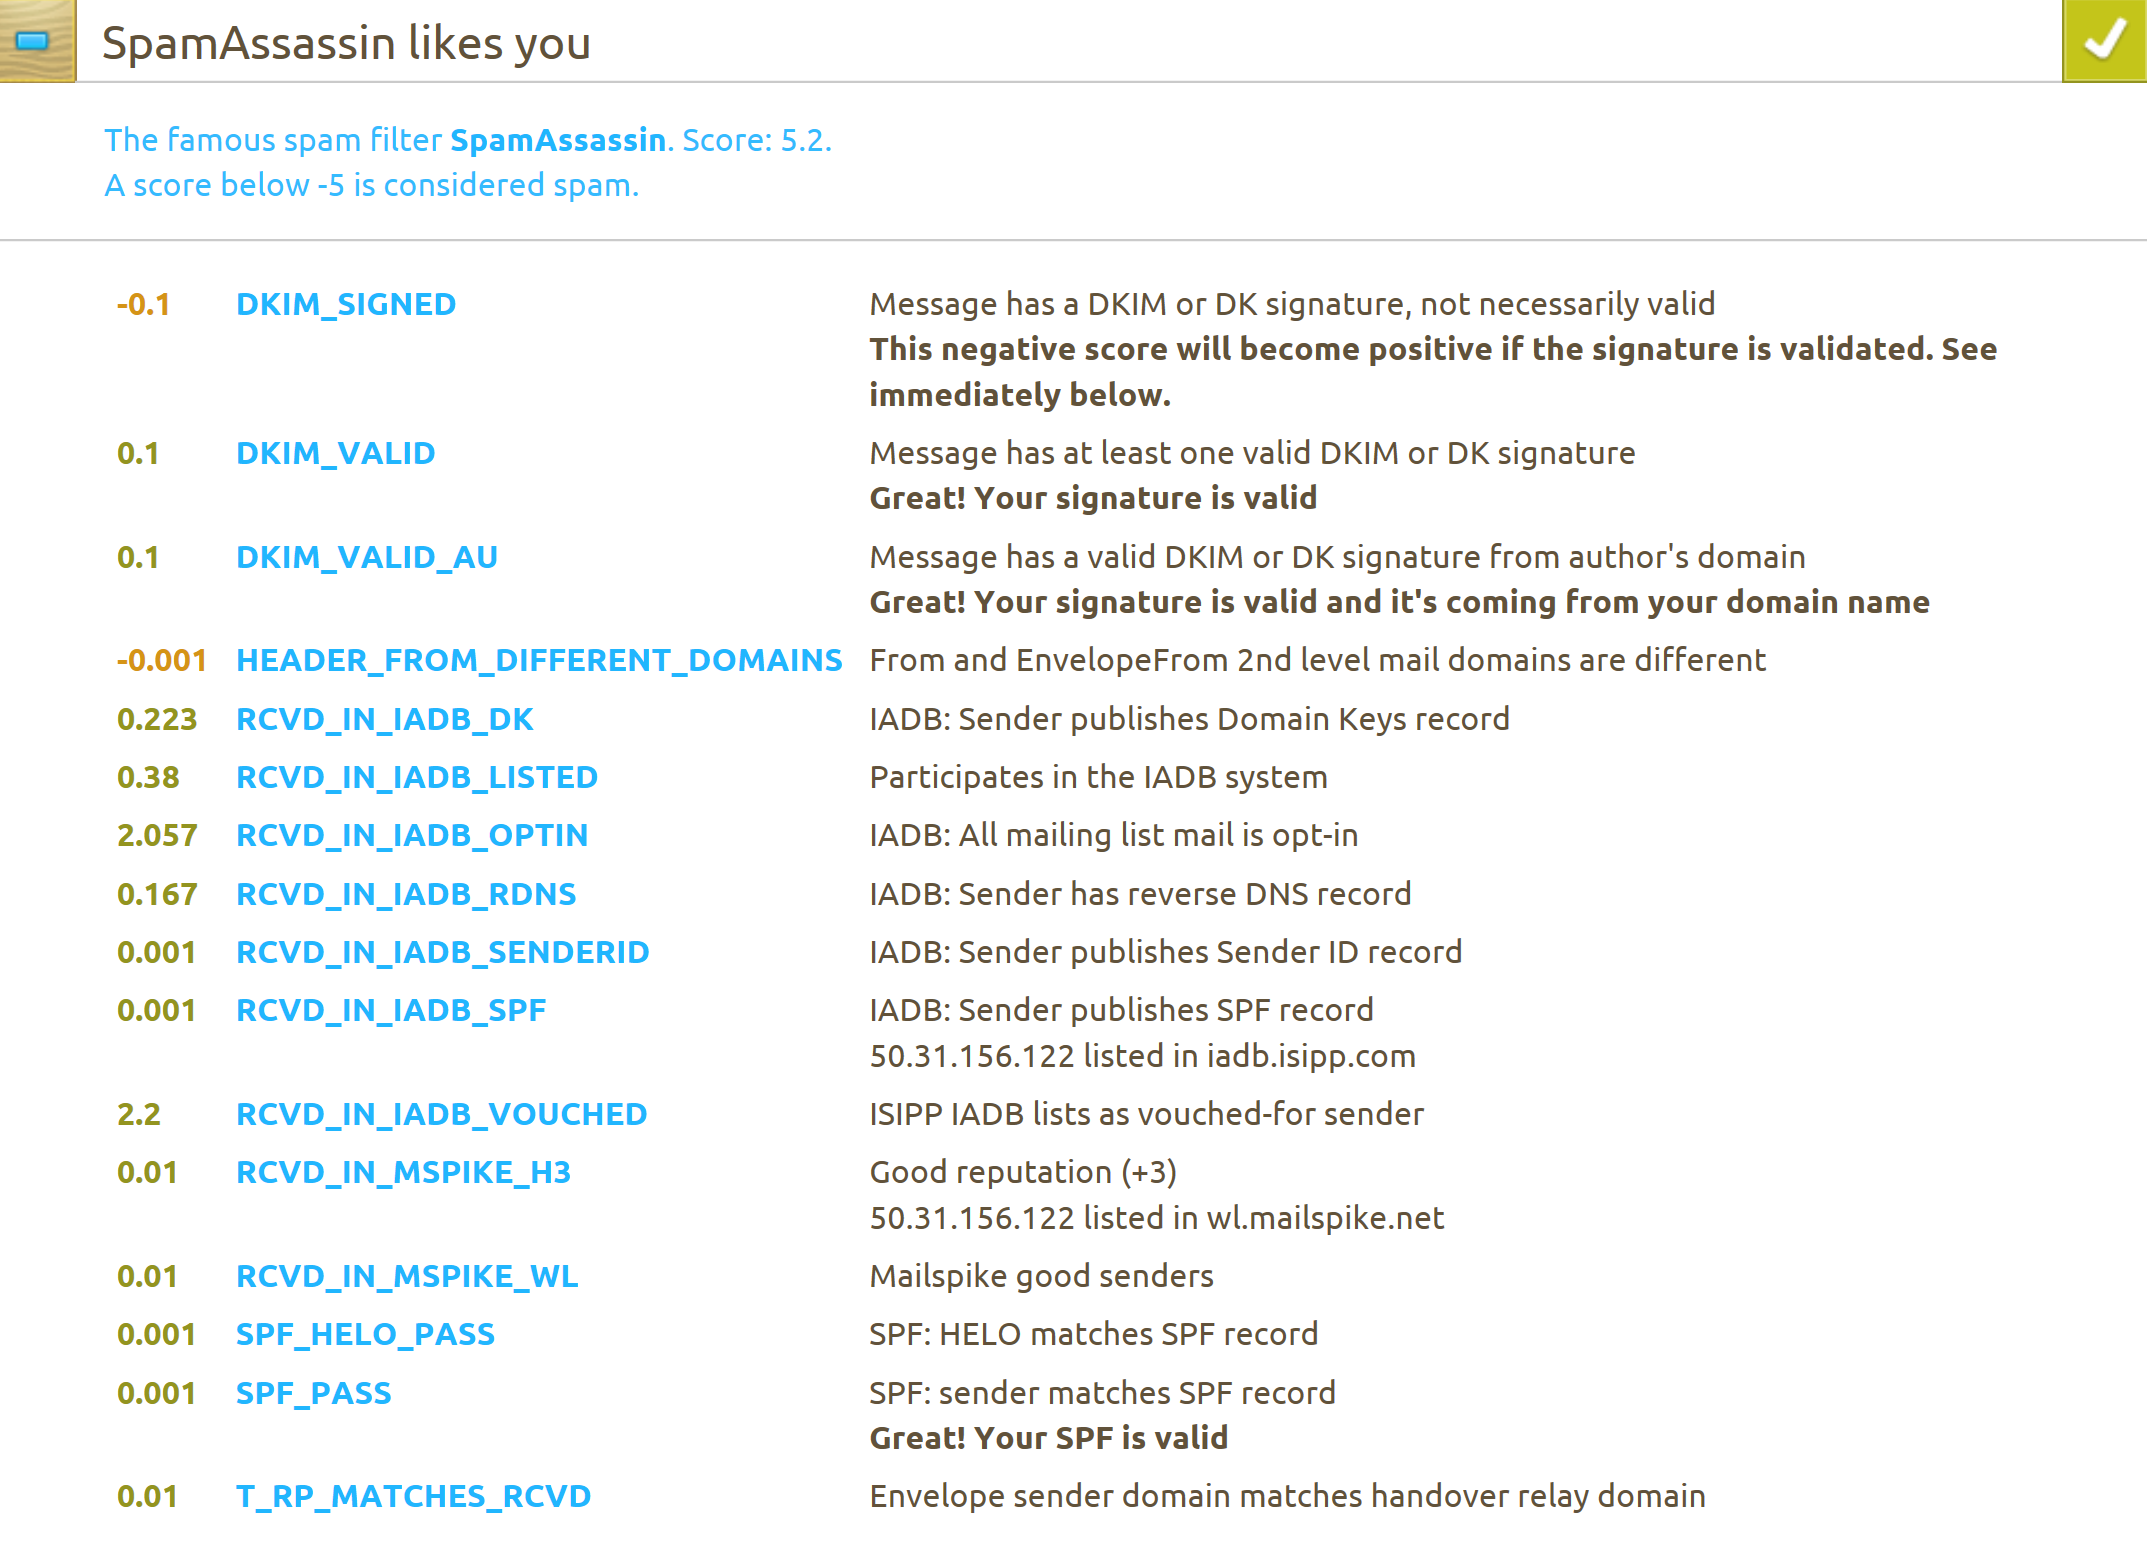
\includegraphics[width=\linewidth]{postmark_spamassassin.png}
	\captionof{figure}{Result of SpamAssassin ran against Postmark (Run on \href{https://www.mail-tester.com/}{Mail-Tester})}
	\label{postmark_spam}
\end{figure}

\begin{figure}
	\centering
	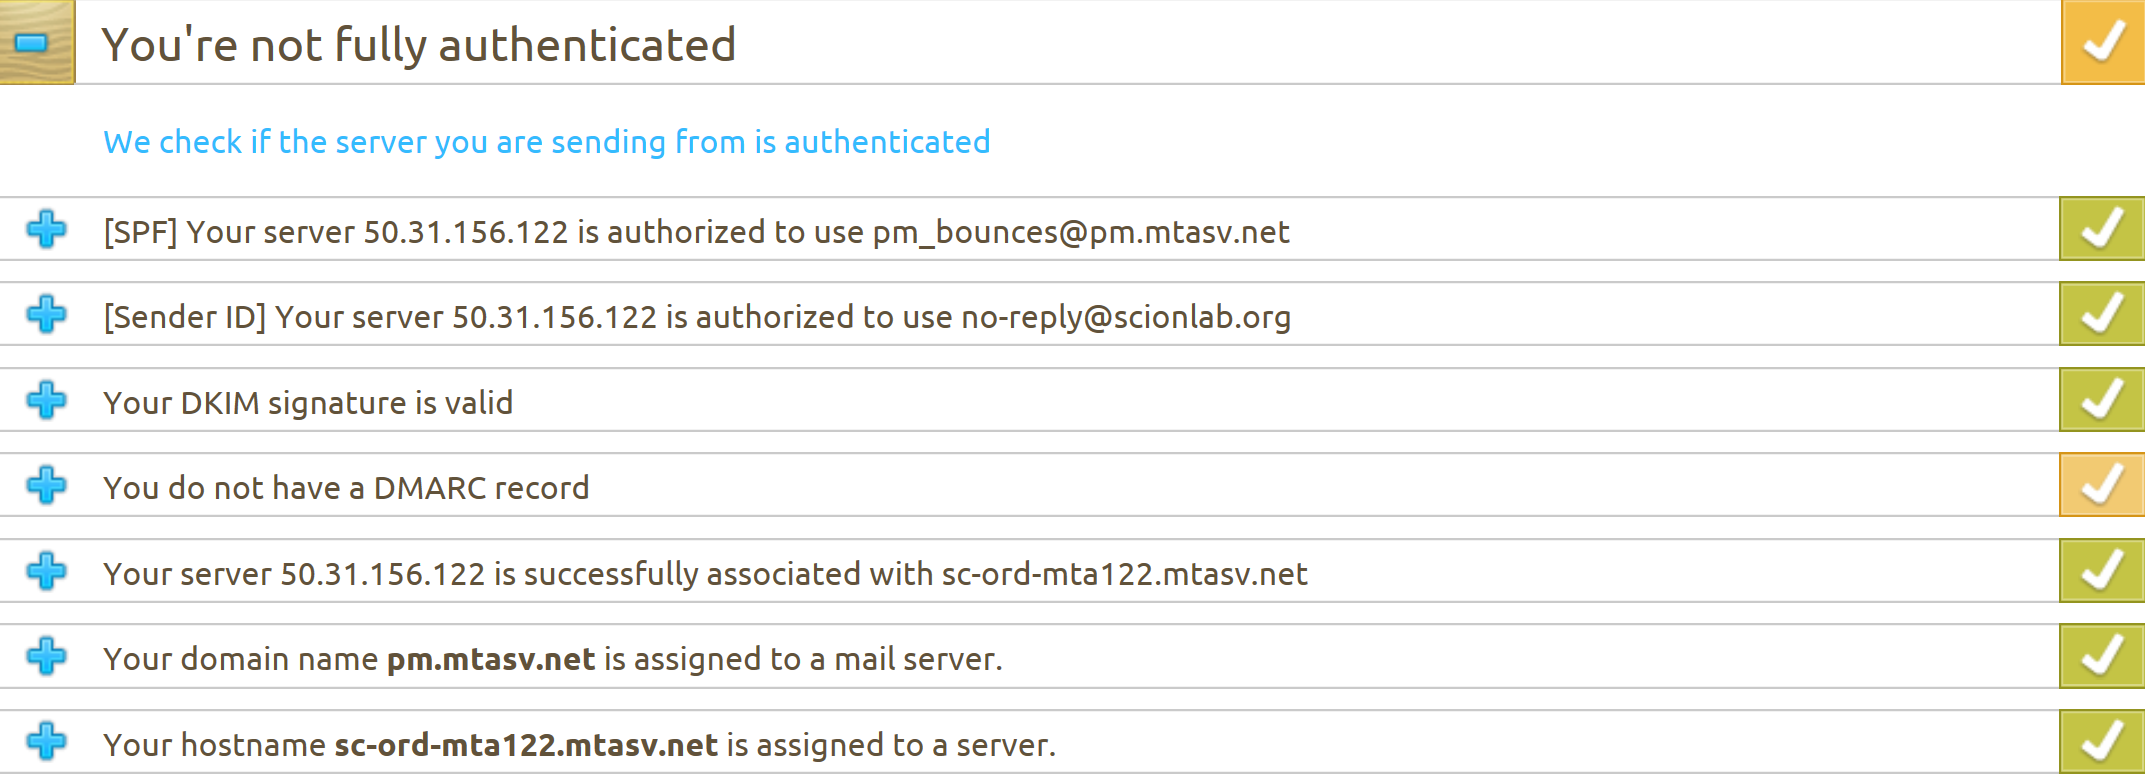
\includegraphics[width=\linewidth]{postmark_auth.png}
	\captionof{figure}{Authentication report for Postmark (Run on \href{https://www.mail-tester.com/}{Mail-Tester})}
	\label{postmark_auth}
\end{figure}

\subsection{Adapted Components}

Apart from the added email package, other components had to be adapted to implement the feature. The following functionality was added:

\subsubsection{User information on Web Interface}
On the web interface, an alert box was integrated on the registration page. Upon successful registration it asks the user to check his emails. Otherwise it displays an error corresponding to the problem that occurred.

\subsubsection{Email creation}
The existing code to register a new user was extended to additionally prepare a personalized email, containing the verification link. This email then gets sent using the email package. The unique identifier contained in the link is stored in the database together with the user information. This allows for a direct mapping between user and identifier.

\subsubsection{Verification API}
A new API was added for handling email address verification requests. This API gets called by the user's web browser when following the confirmation link. Listing \ref{lst_verify_api} shows the signature of the API. \code{uuid} denotes the per-user unique identifier.

\begin{lstlisting}[language=golang, caption={API signature for verifying an email address}\label{lst_verify_api}, float]
//email validation
router.Handle("/api/verifyEmail/{uuid}",loggingChain.ThenFunc(
	registrationController.VerifyEmail))
\end{lstlisting}
%floatplacement=whatever as argument possible

\subsubsection{Handler Function}
A new handler function which gets invoked by the above API call. It checks that the identifier sent in the request is valid and belongs to a user with a not yet verified email address. If the identifier is valid, the corresponding user is set to verified and a confirmation page gets served to the web browser. If not, an error is logged and forwarded to the web browser.

\subsubsection{Confirmation Page}
A confirmation page informing the user about the successful verification process was added to the web interface. This is the page served by the handler function on successful verification. It offers a shortcut to the login page.

\section{Manual User Activation}
\label{impl_user_activation}
The manual user activation feature builds on top of the email verification system. After verifying the email address a user should not immediately be granted access to \lcs. A second verification step is required. The user needs to be activated. To make the process of user activation as automated as possible we distinguish between two cases. Either the user's email address is on a list of pre-defined, trusted domain names. In this case the activation is done automatically. In case the email's domain name is not on the list, the user has to be manually approved by an administrator. Manual activation happens through a newly designed administrator panel added to the web interface. The process with it's two cases is outlined in Figure \ref{acti:dia}. The notification emails sent to administrators and users make use of the new email package introduced for the email verification system.

\begin{figure}
	\centering
	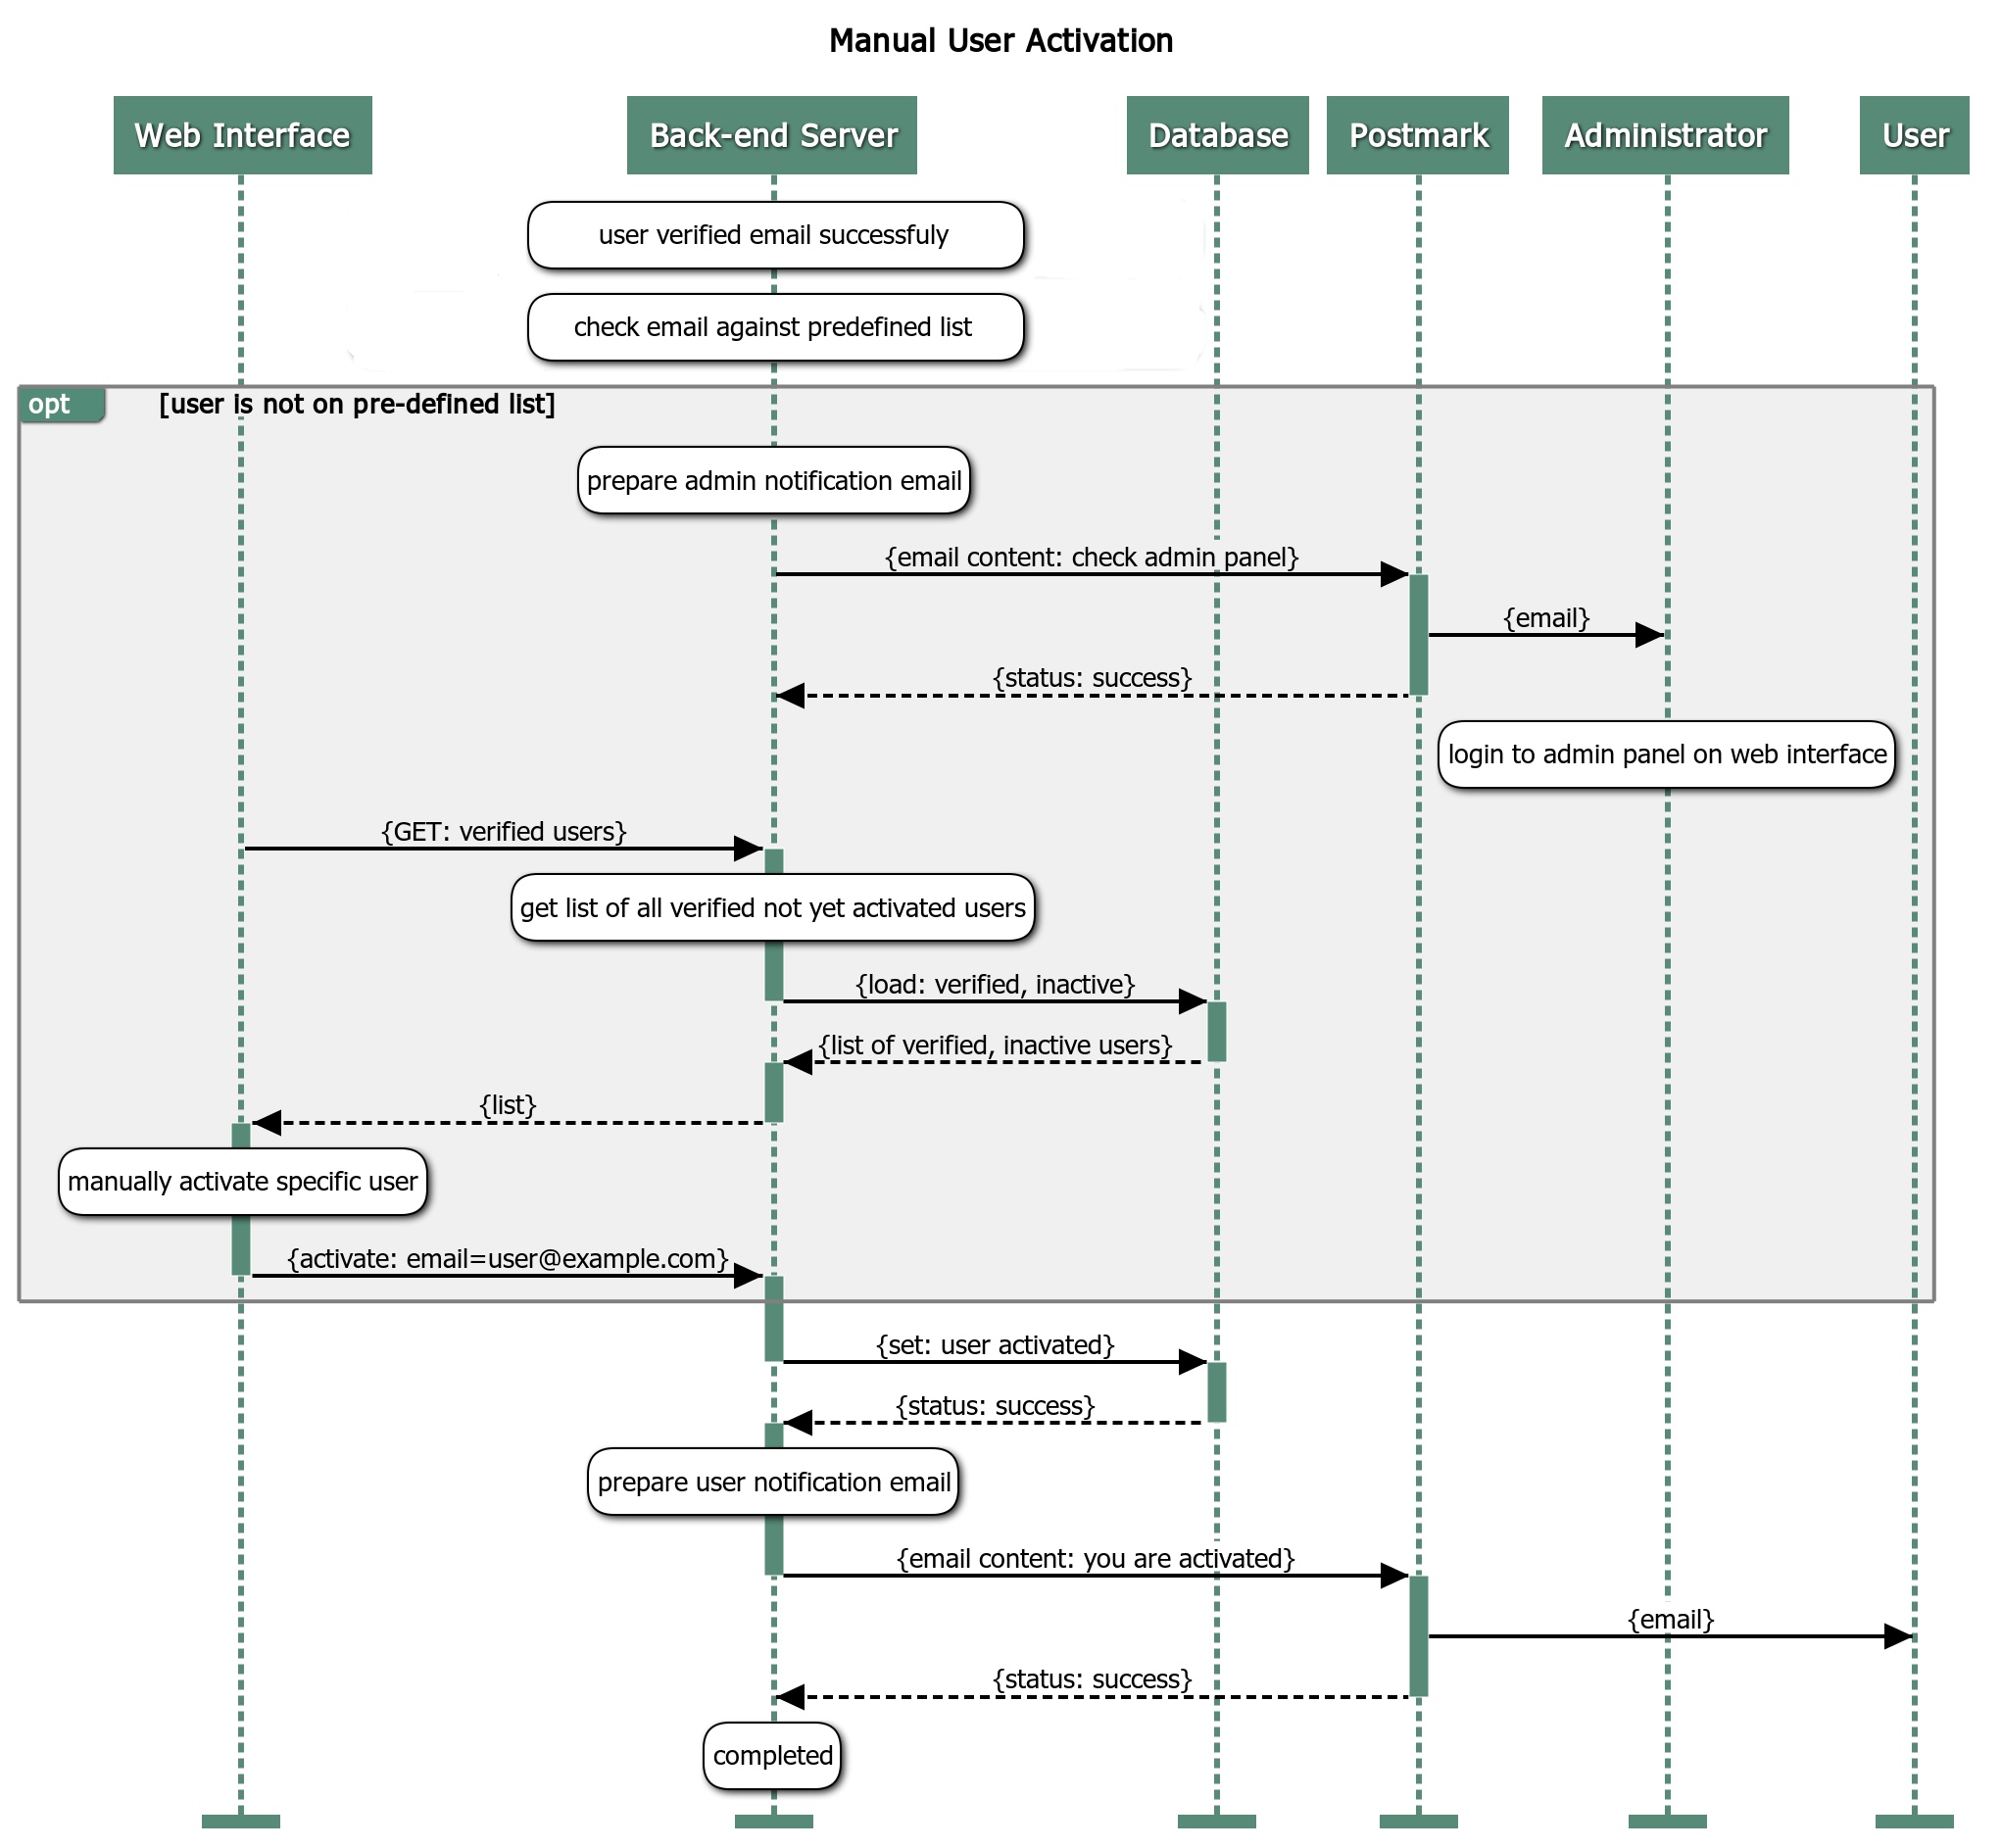
\includegraphics[width=\linewidth]{manual_user_activation.png}
	\captionof{figure}{Sequence diagram showing the messages exchanged for the Manual User Activation feature}
	\label{acti:dia}
\end{figure}

\subsection{Role based access control}
In order to activate a regular user by an administrator the concept of different user groups had to be introduced to \lcs. For this purpose the system was adapted to support a simple role based access control model (RBAC). Instead of granting special rights to individual users each user gets instantiated with a role that reflects the rights this user should possess. This model easily supports many different roles with distinct sets of permissions. However, for the user activation feature only two roles were needed; an administrator role and a regular user role. The regular user role is the role assigned to standard users when signing up through the web interface of \lcs. The administrator role possesses all the permissions of the regular user role and additionally the ability to log in to the administrator panel via the web interface, from where regular users can be activated.

\subsection{Adapted Components}

On top of the changes made to implement the RBAC model the following enhancements were made to support the user activation feature:

\subsubsection{Admin User Creation}
We mentioned above that creating a user through the web interface assigns the regular user role. In order to bootstrap administrator creation, \lcs was extended to accept command line arguments that allow the creation of administrators on system start up. Administrators could then be used to create other administrators. However, such functionality is not in place yet.

\subsubsection{Activation API}
Activating users through the administrator panel requires the web interface to issue two types of requests to the back end server (see Figure \ref{acti:dia}). First, it retrieves a list of all verified, not yet activated users. Then, for a selected user, it issues an activation command. The signature of these two API calls are shown in Listing \ref{lst_acti_api}.

\begin{lstlisting}[language=golang, caption={API signatures for loading unactivated users and for activating users}\label{lst_acti_api}, float]
// user activation
router.Handle("/api/loadUnactivatedUsers", loggingChain.ThenFunc(
	loginController.LoadUnactivatedUsers))
router.Handle("/api/activateUser", loggingChain.ThenFunc(
	loginController.ActivateUser)).Methods("POST")
\end{lstlisting}

\subsubsection{Handler Functions}
Corresponding to the APIs in Listing \ref{lst_acti_api}, \lcs was extended with two new handler functions. \code{LoadUnactivatedUsers} first checks if the request was issued by an administrator. If this is the case it retrieves a list of all verified, inactive users from the database and sends it back in the HTTP response. Otherwise an error is sent to the web interface.

The second handler function, \code{ActivateUser}, performs the same administrator authentication check and, on success, activates the user corresponding to the email address contained in the request. If the authentication fails, the handler responds with an error.

\subsubsection{Email Notifications}
Using the email package introduced in Section \ref{impl_email_package}, new notification emails were added to \lcs:

An email gets sent to all administrators when there are new users waiting to be activated in the administrator panel. This ensures that users who can not be activated automatically are not waiting too long for their activation. This email is sent once there are pending users, rather than for every individual user.

When a user gets manually activated, an email informing about the changed status gets sent to that user. It contains a link to the login page of the web interface.

\subsubsection{Pre-defined List}
In Section \ref{impl_user_activation} we mentioned that users with a trusted email address get activated automatically after they verify their email address. In order to implement this feature, trusted email domain names are collected in a list that comes as part of the \lcs configuration.

The following formats are possible:

\begin{itemize}
	\item example@domain.tld (full email address)
	\item domain.tld (domain \& \fnote{TLD}{Top Level Domain})
	\item sub1...sub2.domain.tld (subdomains \& TLD)
	\item tld (TLD only)
\end{itemize}

Upon successful verification, it is checked whether or not the email is on the list. If the address matches an entry, it is immediately activated. Otherwise the user must go through the manual activation process.


\subsubsection{Administrator Panel}
A new administrator panel was added to the web interface. It displays a table containing all verified, inactive users together with their relevant information like name, email address and organisation. Individual users can be activated via an activation button.

\subsubsection{Confirmation Page}
The confirmation page displayed when users follow the email verification link was revamped to provide users who can not be activated automatically with information about the extended activation process.

\section{CAPTCHA Integration}
\label{impl_capt}

Fake accounts can negatively impact the performance of a system, and with email sending involved in the registration process, bots can abuse \lcs for spamming. As counter measurement against such malicious behaviour, a CAPTCHA was placed on the registration page. The interaction of users with the CAPTCHA and its overall integration into \lcs can be seen in Figure \ref{capt:dia}.
  
\begin{figure}
	\centering
	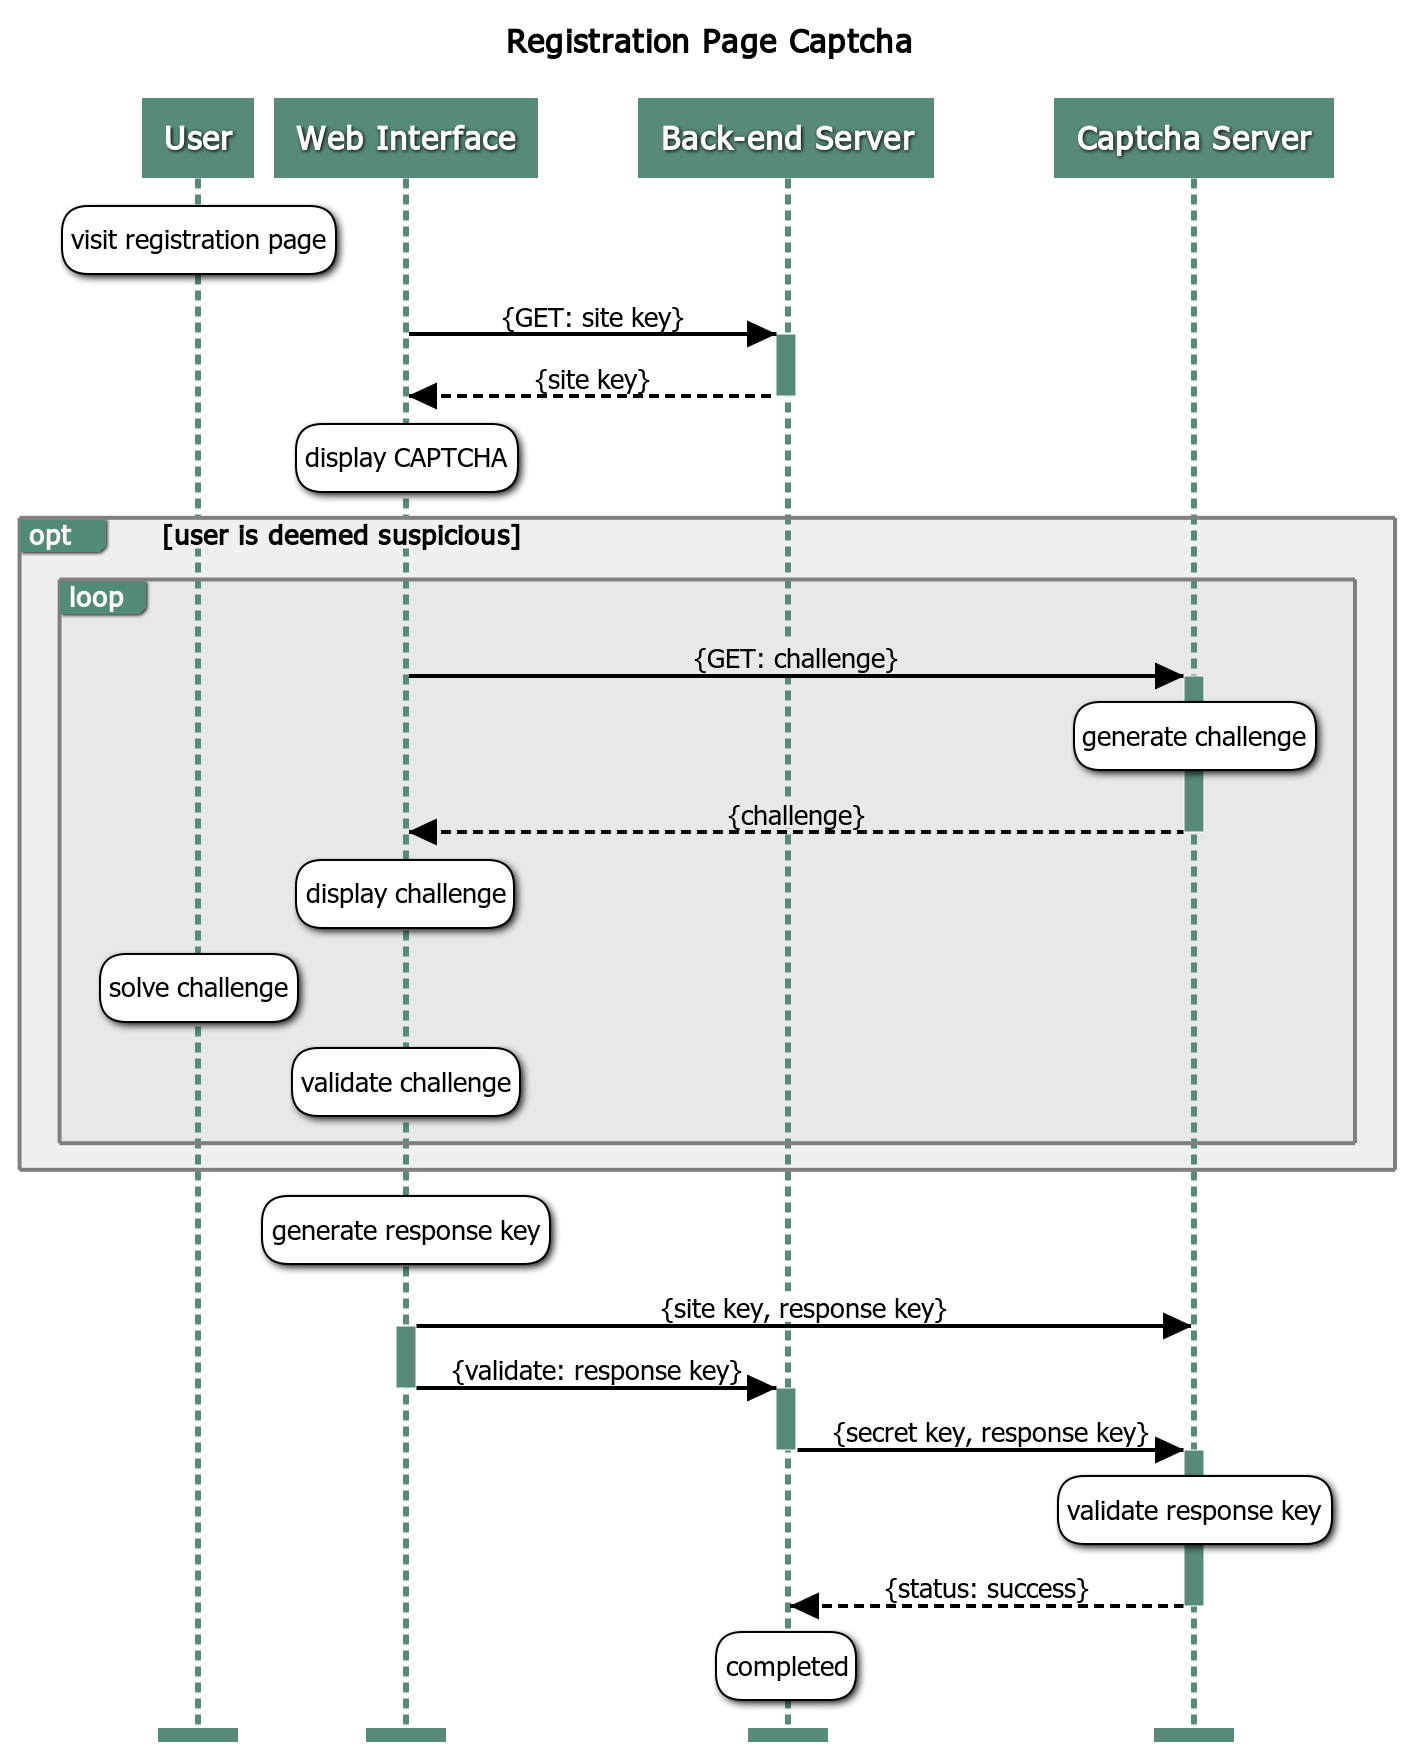
\includegraphics[width=\linewidth]{captcha.png}
	\captionof{figure}{Sequence diagram showing the exchanged messages for the CAPTCHA implementation}
	\label{capt:dia}
\end{figure}


\subsection{Google reCAPTCHA}
For \lcs, Google \fnurl{reCAPTCHA}{https://www.google.com/recaptcha/intro/android.html} was chosen as CAPTCHA provider for a variety of reasons: Since reCAPTCHA is the most popular CAPTCHA service many users will be familiar with how it works. \cite{google_recaptcha} Also, thanks to its advanced risk analysis which observes a user's interaction with the website to infer whether a user is human, often users are not forced to solve a challenge to pass the Turing test. A mere click on a check box is enough to pass.  \cite{google_recaptcha} This effortless verification for human users complies with the non-functional requirements of \lcs outlined in Section \ref{non-func_req}. 
Furthermore, reCAPTCHA is very well supported and documented by Google which makes implementation straight forward.

reCAPTCHA uses a set of keys to fulfill its task. The web page containing the reCAPTCHA must be registered to obtain a site key and a secret key. The site key is used to create reCAPTCHA response keys for users passing the Turing test. This response key then gets verified by sending it to a reCAPTCHA server together with the secret key. Additionally, the reCAPTCHA server provides the reCAPTCHA widget on the web page with challenges to be solved. 

\subsection{Adapted Components}

In order to implement the reCAPTCHA for the registration page of the web interface the following changes had to be made to the system:

\subsubsection{CAPTCHA API}

On the web interface reCAPTCHA must be instantiated with the site key corresponding to the web page it is placed on. When the page loads this site key is retrieved via an API call from the back end server. This offers the convenience of having all keys stored in the main configuration file of \lcs rather than hard coding the site key into the web page. Like this, if new keys need to be installed or \lcs is deployed onto another machine, only the configuration file has to be changed. 

The response key gets appended to the user information as an attribute and is sent using the existing registration API call to the back end server where it is validated together with other user information.

The described endpoints are shown in Listing \ref{lst_captcha_api}

\begin{lstlisting}[language=golang, caption={API signatures for registering users and loading the captcha site key}\label{lst_captcha_api}, float]
// user registration
router.Handle("/api/captchaSiteKey", loggingChain.ThenFunc(
	registrationController.LoadCaptchaSiteKey))
router.Handle("/api/register", loggingChain.ThenFunc(
	registrationController.Register)).Methods("POST")
\end{lstlisting}

\subsubsection{Handler Functions}

The newly added \code{LoadCaptchaSiteKey} handler retrieves the site key from the configuration and hands it over to the web interface where it is used to instantiate the reCAPTCHA.

When a user submits his registration information, the existing \code{Register} handler is triggered. It reads the user data, including the response key, from the request and performs validity checks on the submitted information. The following new check was added to this phase:
The site key is sent together with the secret key to the reCAPTCHA sever, which in turn verifies whether or not the response key is valid for the site specified by the secret key. Here, communication with the reCAPTCHA server is done using the third party \fnurl{haisum/recaptcha}{https://github.com/haisum/recaptcha} package. If all checks pass, the user's information is stored in the database.

\subsubsection{CAPTCHA Widget on Registration Page}

Using the \fnurl{VividCortex/angular-recaptcha}{https://github.com/VividCortex/angular-recaptcha} AngularJS directive, the reCAPTCHA widget was placed on the registration page. Solving the reCAPTCHA was made mandatory for sending registration data to the back end.

\section{CircleCI Integration}
\label{impl_ci}

In Section \ref{archi:ci} we talked about CircleCI and how it helps with the software verification process. Every time a pull request is updated with new code CircleCI runs a defined suite of tests in the cloud. For this to work CircleCI must know about the project environment, what dependencies are used and what tests it has to run. This information is pulled from a configuration file that resides in a special folder inside the \lcs code base. These configurations are processed and used to create a minimal, virtual environment in the CircleCI cloud, which is able to run the code to be tested. The contents of the configuration file is shown in Listing \ref{lst_ci}.

The following subsections describe how CircleCI is set up in order to run the test suite. 

\lstinputlisting[language=yaml,caption={CircleCI project configurations}\label{lst_ci}, float]{code/ci.yml}

\subsection{Environment}
The easiest way to set up the required environment is to use a pre-defined \fnoteurl{Docker}{https://www.docker.com/}{Docker bundles software in isolated containers, then runs these containers on a host system using virtualization} image that comes bundled with all the tools needed for the testing and debugging process.

As can be seen on line 6 and 12 in Listing \ref{lst_ci}, two Docker images are used:
The \code{circleci/golang:1.8} image is an image built by CircleCI specifically for testing Go code. It comes with the Go 1.8 environment and numerous other useful tools, such as Git and SSH, pre-installed.

\code{circleci/mysql:latest} additionally installs the latest version of MySQL in the test environment, which is crucial since tests involve storing to and loading from the database. This image also allows setting up the database in a way such that it conforms to what \lcs is expecting. (see lines 8 to 10 of Listing \ref{lst_ci})

\subsection{Dependencies}
\lcs uses many dependencies which all need to be installed for tests to run successfully. Dependencies are downloaded using the Go command \code{go get -v -t -d ./...}. This downloads all needed packages and writes the name of each package to the test log.

\subsection{Testing}
\code{go test -v ./...} looks for all test files in the code base and then runs the test cases one by one. For each test case it writes status information to the log file stating whether the test failed or not. In case of failure, a corresponding error message is logged as well.

\section{Deployment with Ansible}
\label{impl:ansi}

In Section \ref{archi:ansi} we described how Ansible supports the deployment process. As with CircleCI, Ansible needs instructions to put the target machine into the right state and to deploy \lcs correctly. The most important configurations are described below.


\lstinputlisting[language=yaml, linerange={1-20}, caption={Excerpt of Ansible tasks, used to set up \lcs}\label{lst_ansi_tasks}, float]{code/ansi_tasks.yml}

\begin{lstlisting}[language=yaml, caption={Excerpt of the Ansible parameter file used for \lcs}\label{lst_ansi_param}, float]
mysql_db: scion_coord_test
mysql_pass: development_pass
\end{lstlisting}


\subsection{Hosts}
The host configuration file contains sections for different roles to deploy. Within each section, the addresses of the machines assigned to this role are specified; therefore creating a one-to-many relation between roles and machines.

In the case of \lcs there is only one role, as the complete architecture runs on a single machine.
However, by specifying multiple addresses, the service could easily be replicated for redundancy.

\subsection{Files}
Ansible is capable of copying entire files to a target machine. In \lcs this is used to apply SSH keys and a \fnote{sudoers file}{A file containing rules that users must obey when the sudo command is used} to the deployment environment. This sets up the environment with the necessary user account permissions, required to run \lcs.

\subsection{Parameters}
Certain parameters used in tasks are confidential, do change frequently or are not the same for every target machine. To avoid duplication of playbooks, Ansible allows the use of place holders in tasks.

For simplicity, place holders used in \lcs are compiled in a dedicated parameter file, together with their corresponding values. Lines 13 and 15 of Listing \ref{lst_ansi_tasks} show how place holders are used in a task to confidentially set the password for the MySQL root user. Listing \ref{lst_ansi_param} shows the corresponding excerpt of the parameter file.

\subsection{Tasks}
Ansible runs for each target machine a set of tasks (a playbook), dependant on the assigned role. If tasks are written carefully, the process of running them is idempotent, which means that running the tasks multiple times has no further effect. Idempotence is one of the core concepts of Ansible. It allows tasks to be written in a descriptive way, such that they only get executed when the current state of the machine violates the desired end state. This speeds up the deployment process and prevents data loss caused by writing files which already exist. After completing all tasks, the target machine is in a state that conforms to the state described by the playbook.

Tasks for deploying \lcs consist of installing required packages, setting up the database, applying SSH keys and checking out the code base. Listing \ref{lst_ansi_tasks} shows an excerpt of the playbook used to deploy \lcs. Lines 2-8 show how required packages are installed. As described above, if a package already exists it will not be downloaded again. This speeds up the deployment. Similarly, tasks for setting up the database (lines 10-20) only run when needed to reach the end state, preventing data loss in case the database already exists. % Updated components / New components
\chapter{Evaluation}

 % Evaluation
\chapter{Conclusion}


  % Conclusion

\appendix

\chapter{Security and Maintainability Enhancements}
\label{misc}


\backmatter

\bibliography{refs}
\bibliographystyle{unsrtnat}

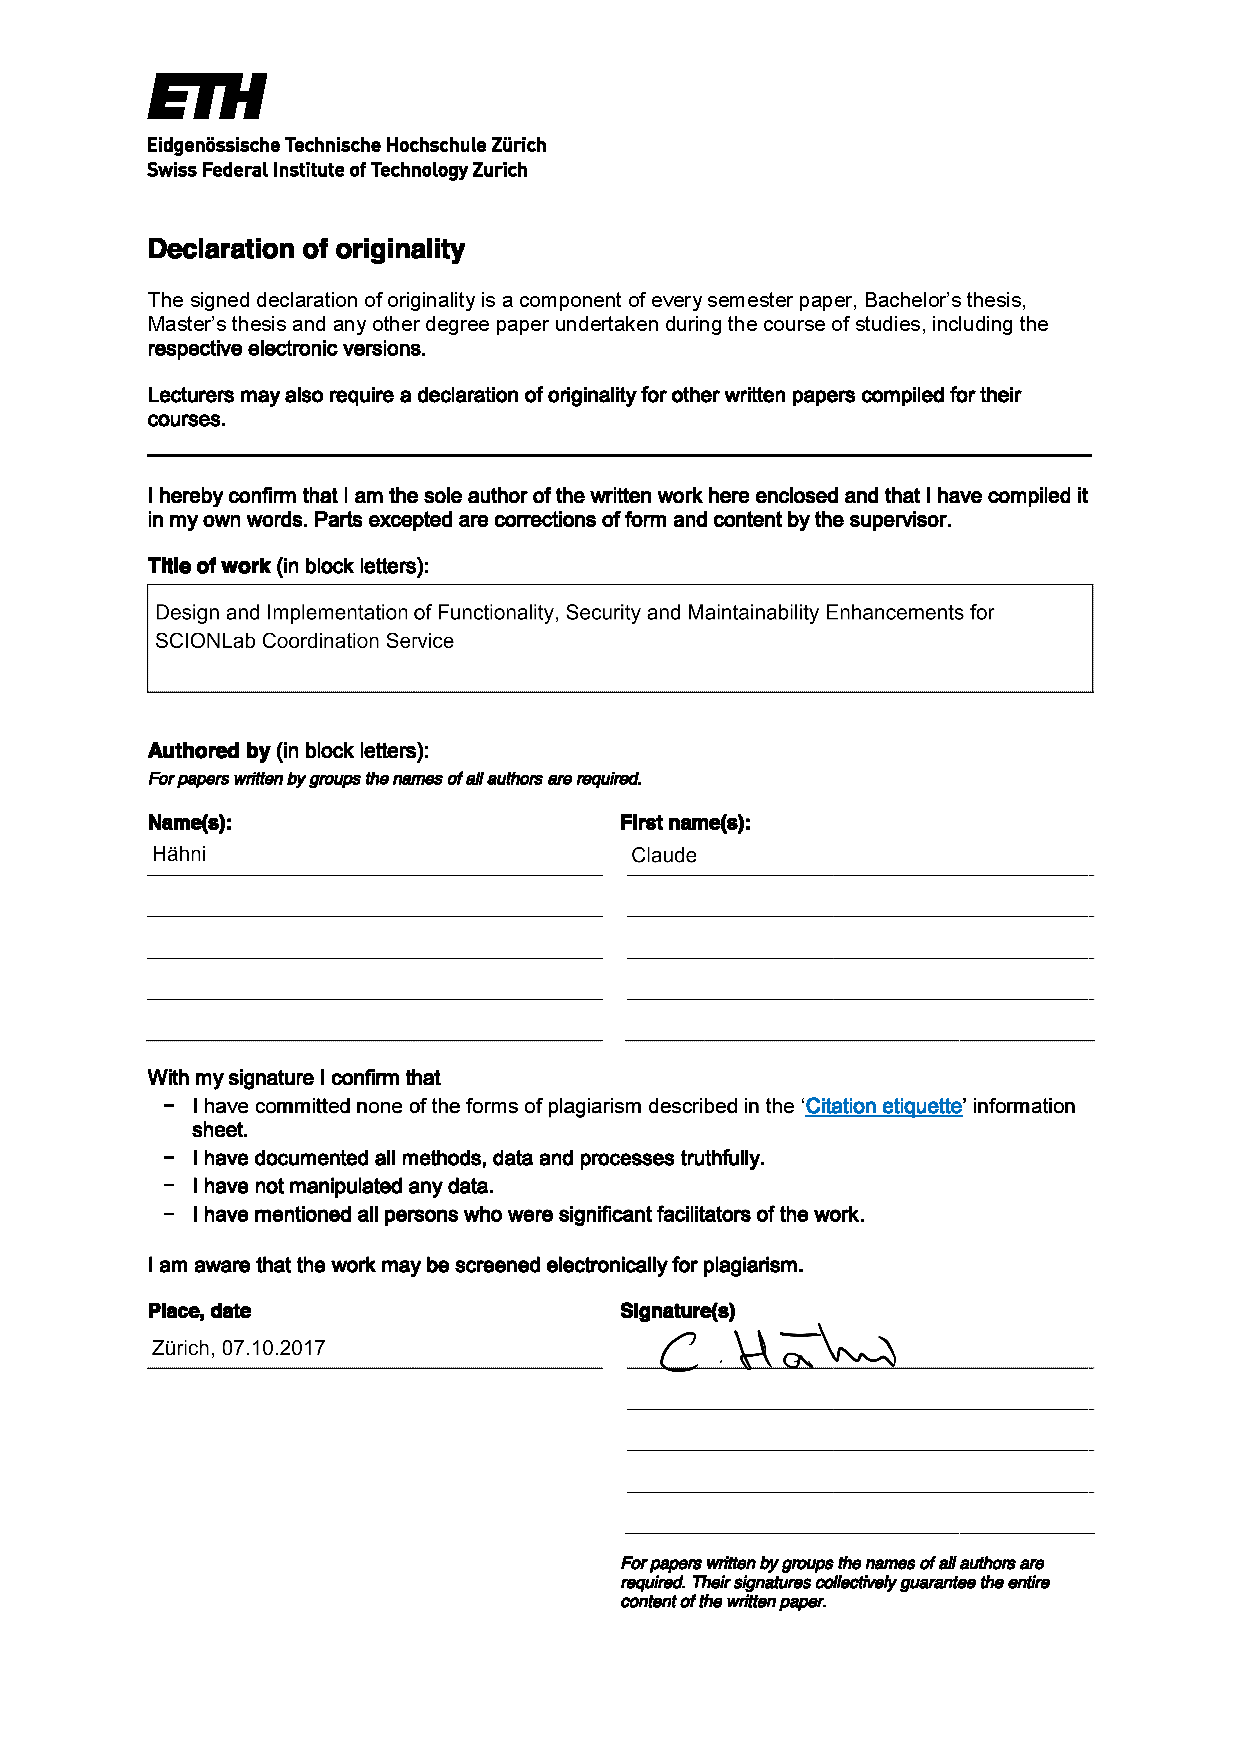
\includepdf[pages={-}]{declaration-originality-filled.pdf}

\end{document}
